\documentclass[
    ngerman,%globale Übergabe der Hauptsprache
%	logofile=example-image, %Falls die Logo Dateien nicht vorliegen
    authorontitle=true,
]{bfhbeamer}

% Used for images
\usepackage{graphicx}
\usepackage{tikz}
\usetikzlibrary{shapes.geometric} % for hexagonal shapes
% Define a new command for creating hexagon-shaped images
\newcommand{\hexagonimage}[2][]{
    \begin{tikzpicture}
        \node[regular polygon, regular polygon sides=6, draw, inner sep=0pt, minimum width=3cm, path picture={
            \node at (path picture bounding box.center) {
                \includegraphics[width=3cm,#1]{#2}
            };}] {};
    \end{tikzpicture}
}


%\usepackage[main=ngerman]{babel}

% Der folgende Block ist nur bei pdfTeX auf Versionen vor April 2018 notwendig
%\usepackage{iftex}
%\ifPDFTeX
%\usepackage[utf8]{inputenc}%kompatibilität mit TeX Versionen vor April 2018
%\fi


%Makros für Formatierungen der Doku
%Im Allgemeinen nicht notwendig!
%\let\code\texttt

\title{URL-Archiver}
\subtitle{Final Presentation}
\author[N. Dora \and A. Vejseli \and K. Wampfler]{N. Dora, A. Vejseli, K. Wampfler}
\institute{School of Engineering and Computer Science}
\titlegraphic*{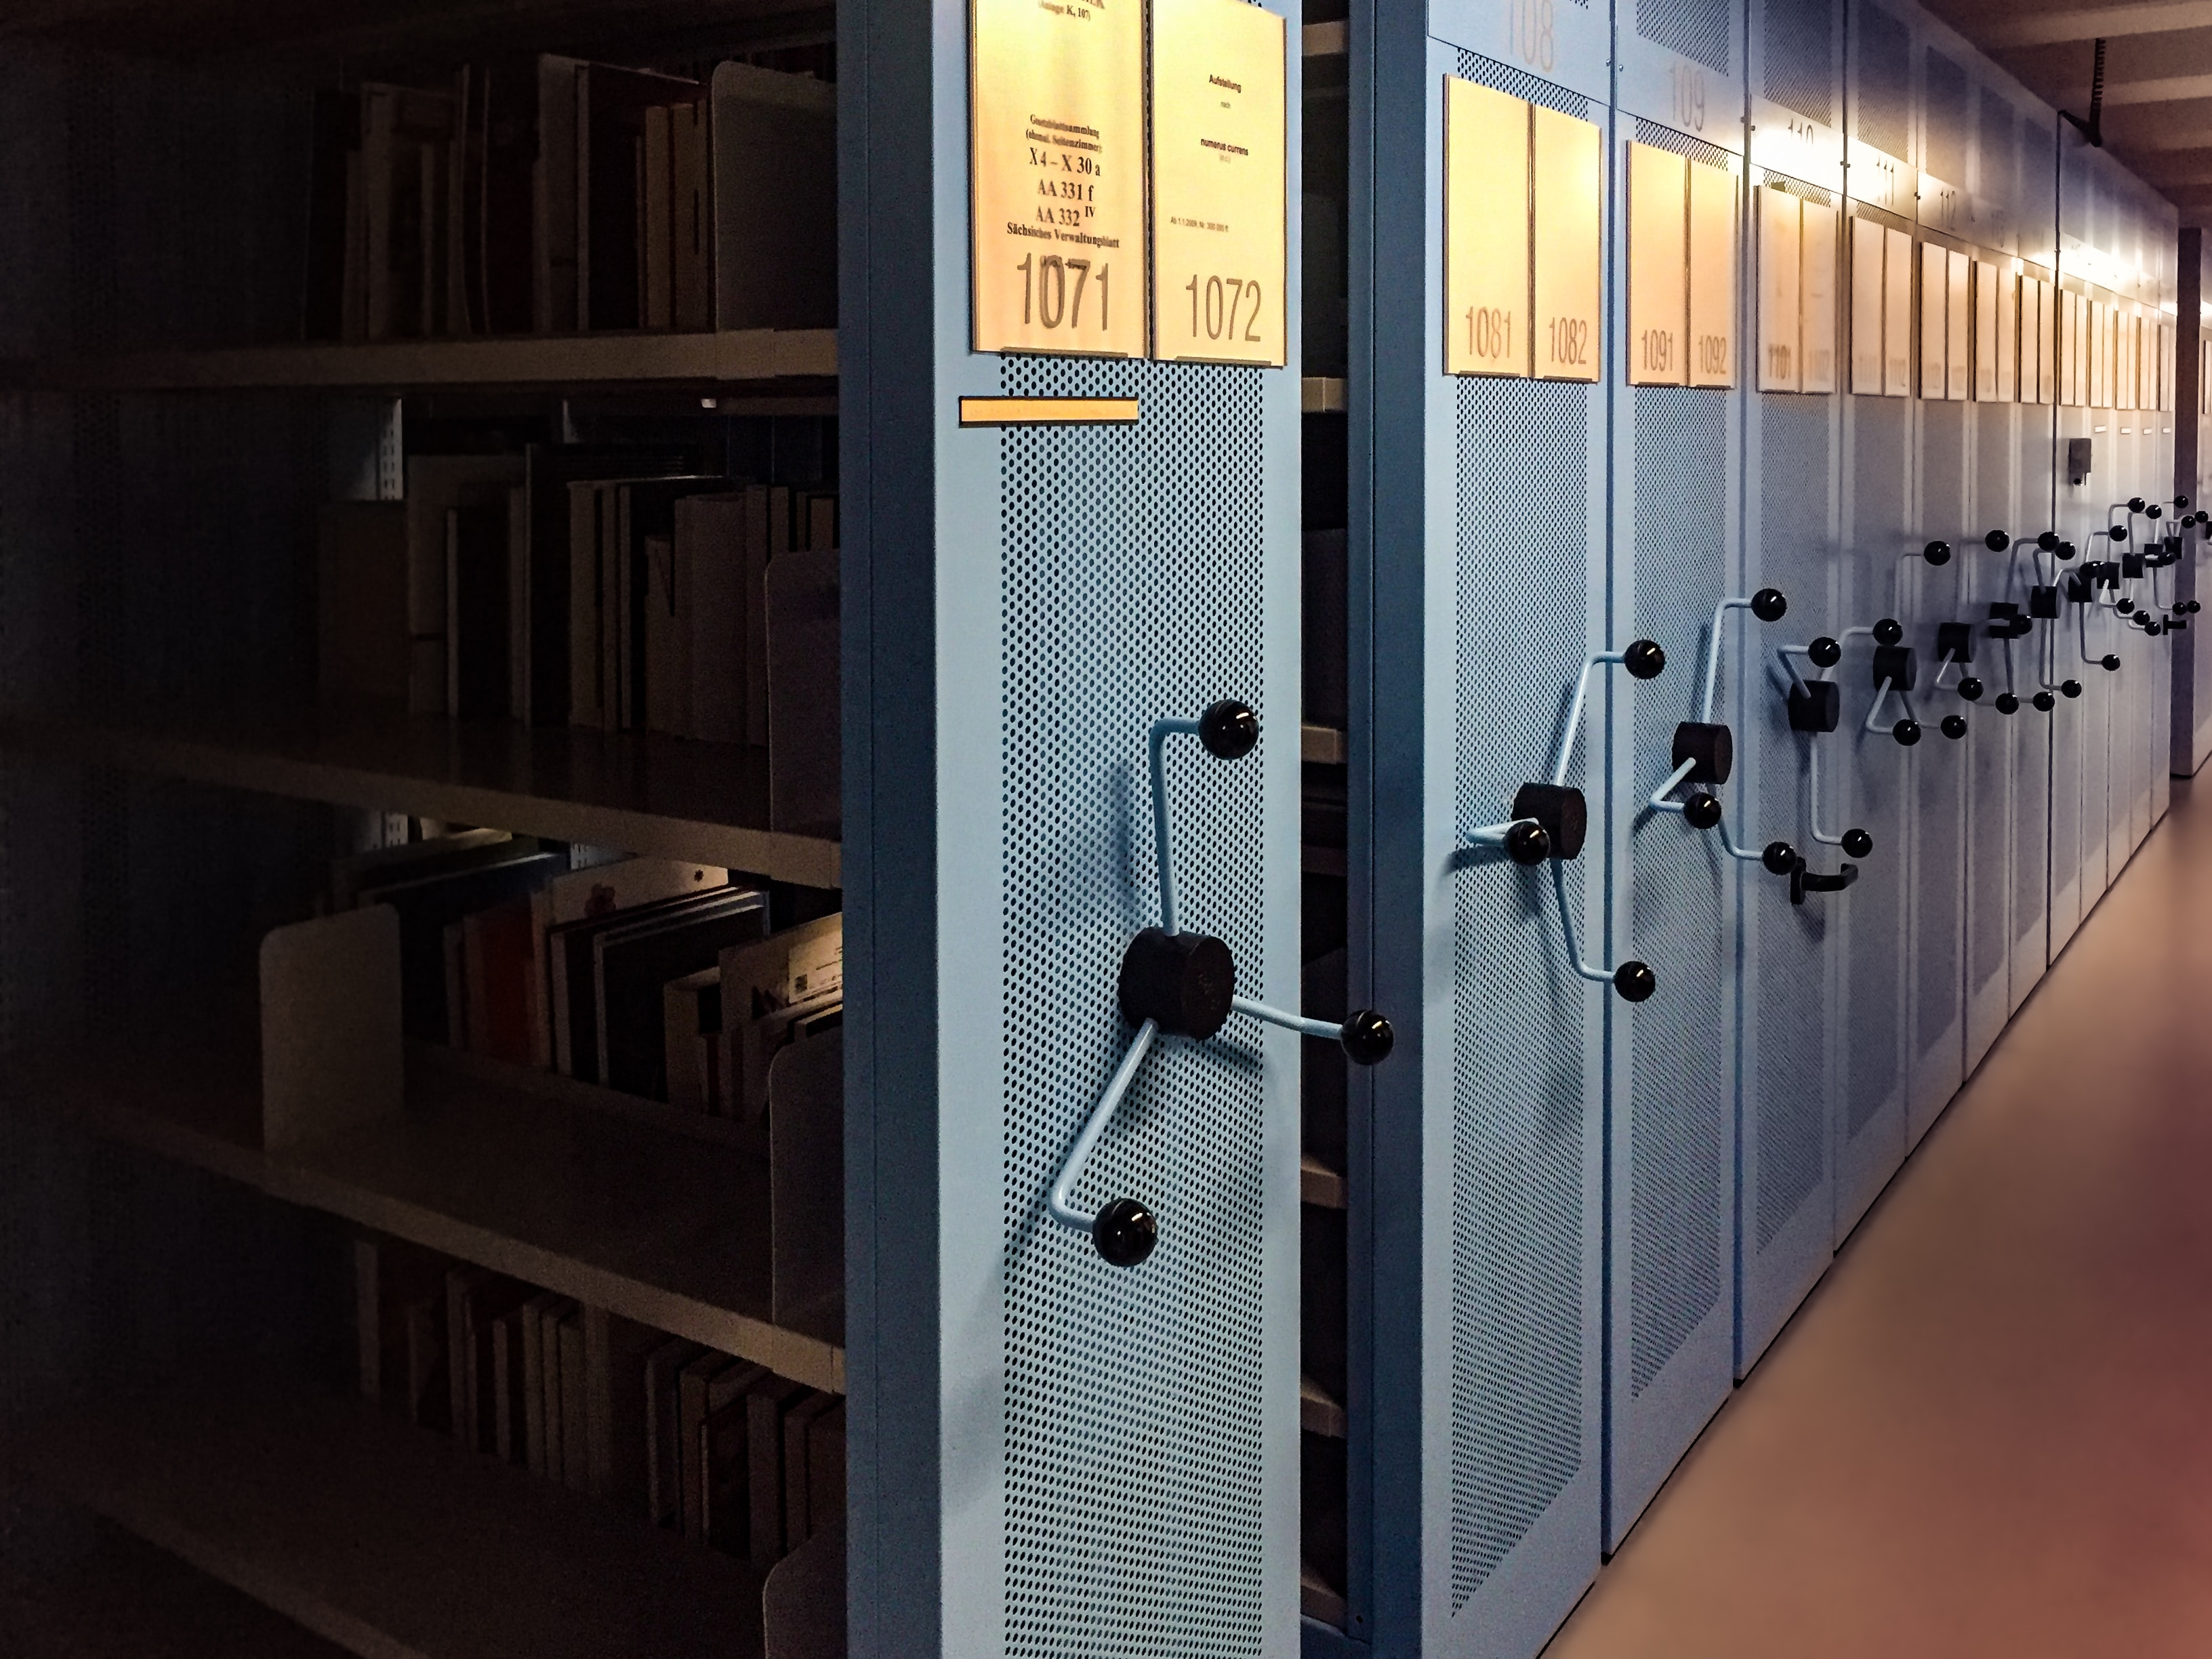
\includegraphics{pictures/archive-title-image}}%is only used with BFH-graphic and BFH-fullgraphic

%Activate the output of a frame number:
\setbeamertemplate{page number in head/foot}[framenumber]

\begin{document}

    \setbeamertemplate{title page}[BFH-fullgraphic]
    \maketitle



    \begin{frame}{Table of Content}
        \framesubtitle{Topics Covered}
        \begin{columns} % Start the columns environment
            \begin{column}{0.4\textwidth} % Define the width of the left column
                %\setcounter{tocdepth}{1}
                \tableofcontents
            \end{column}
            \begin{column}{0.6\textwidth} % Define the width of the left column
                \begin{center}
                    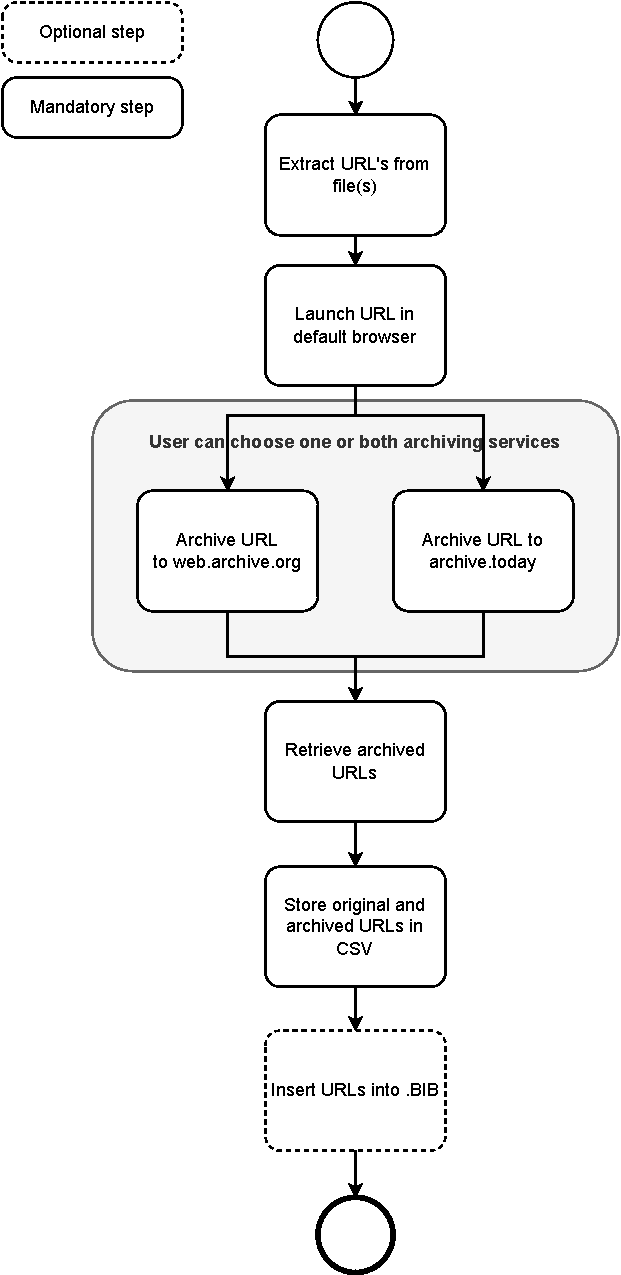
\includegraphics[width=0.3\textwidth]{figures/process_model-simple-vertikal}
                    %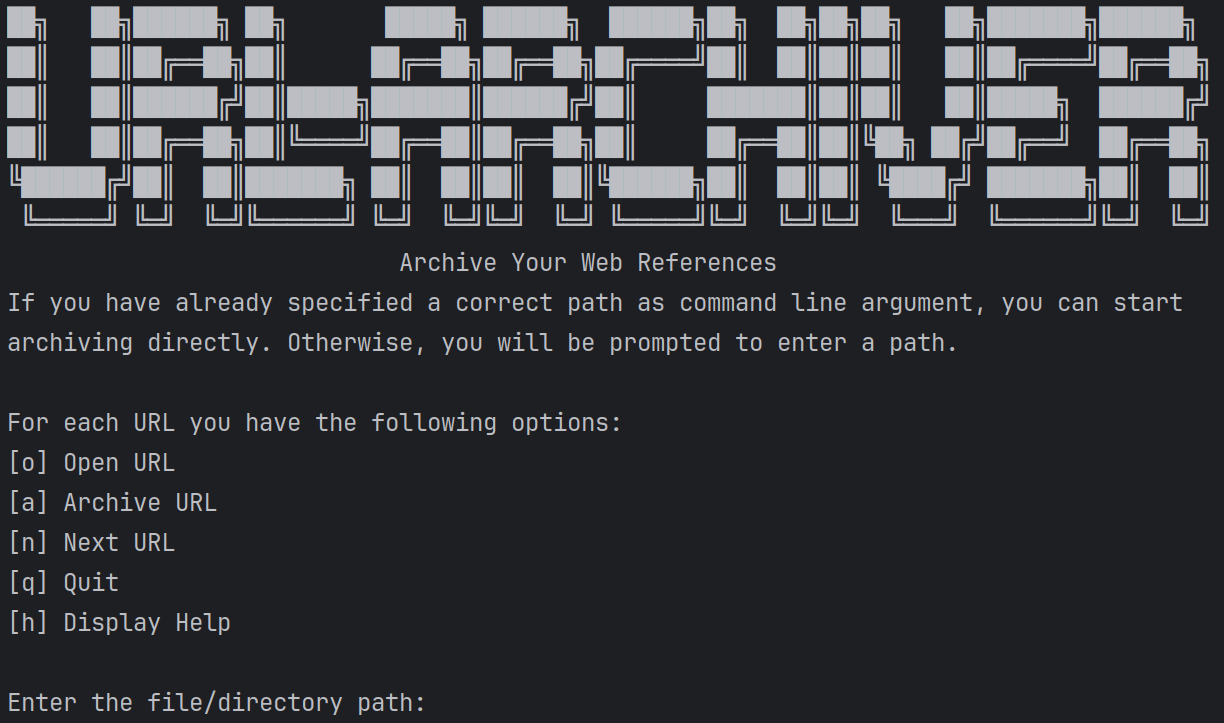
\includegraphics[width=0.6\textwidth]{pictures/URL_Archiver_Screenshot}
                \end{center}
            \end{column}
        \end{columns}
    \end{frame}

	% Template slide
	    \begin{frame}{Template}
		% Nicolin
		\framesubtitle{Template with columns}
		\begin{columns} % Start the columns environment
			\begin{column}{0.7\textwidth} % Define the width of the left column
				
			\end{column}
			\begin{column}{0.3\textwidth} % Define the width of the left column
				\begin{center}
					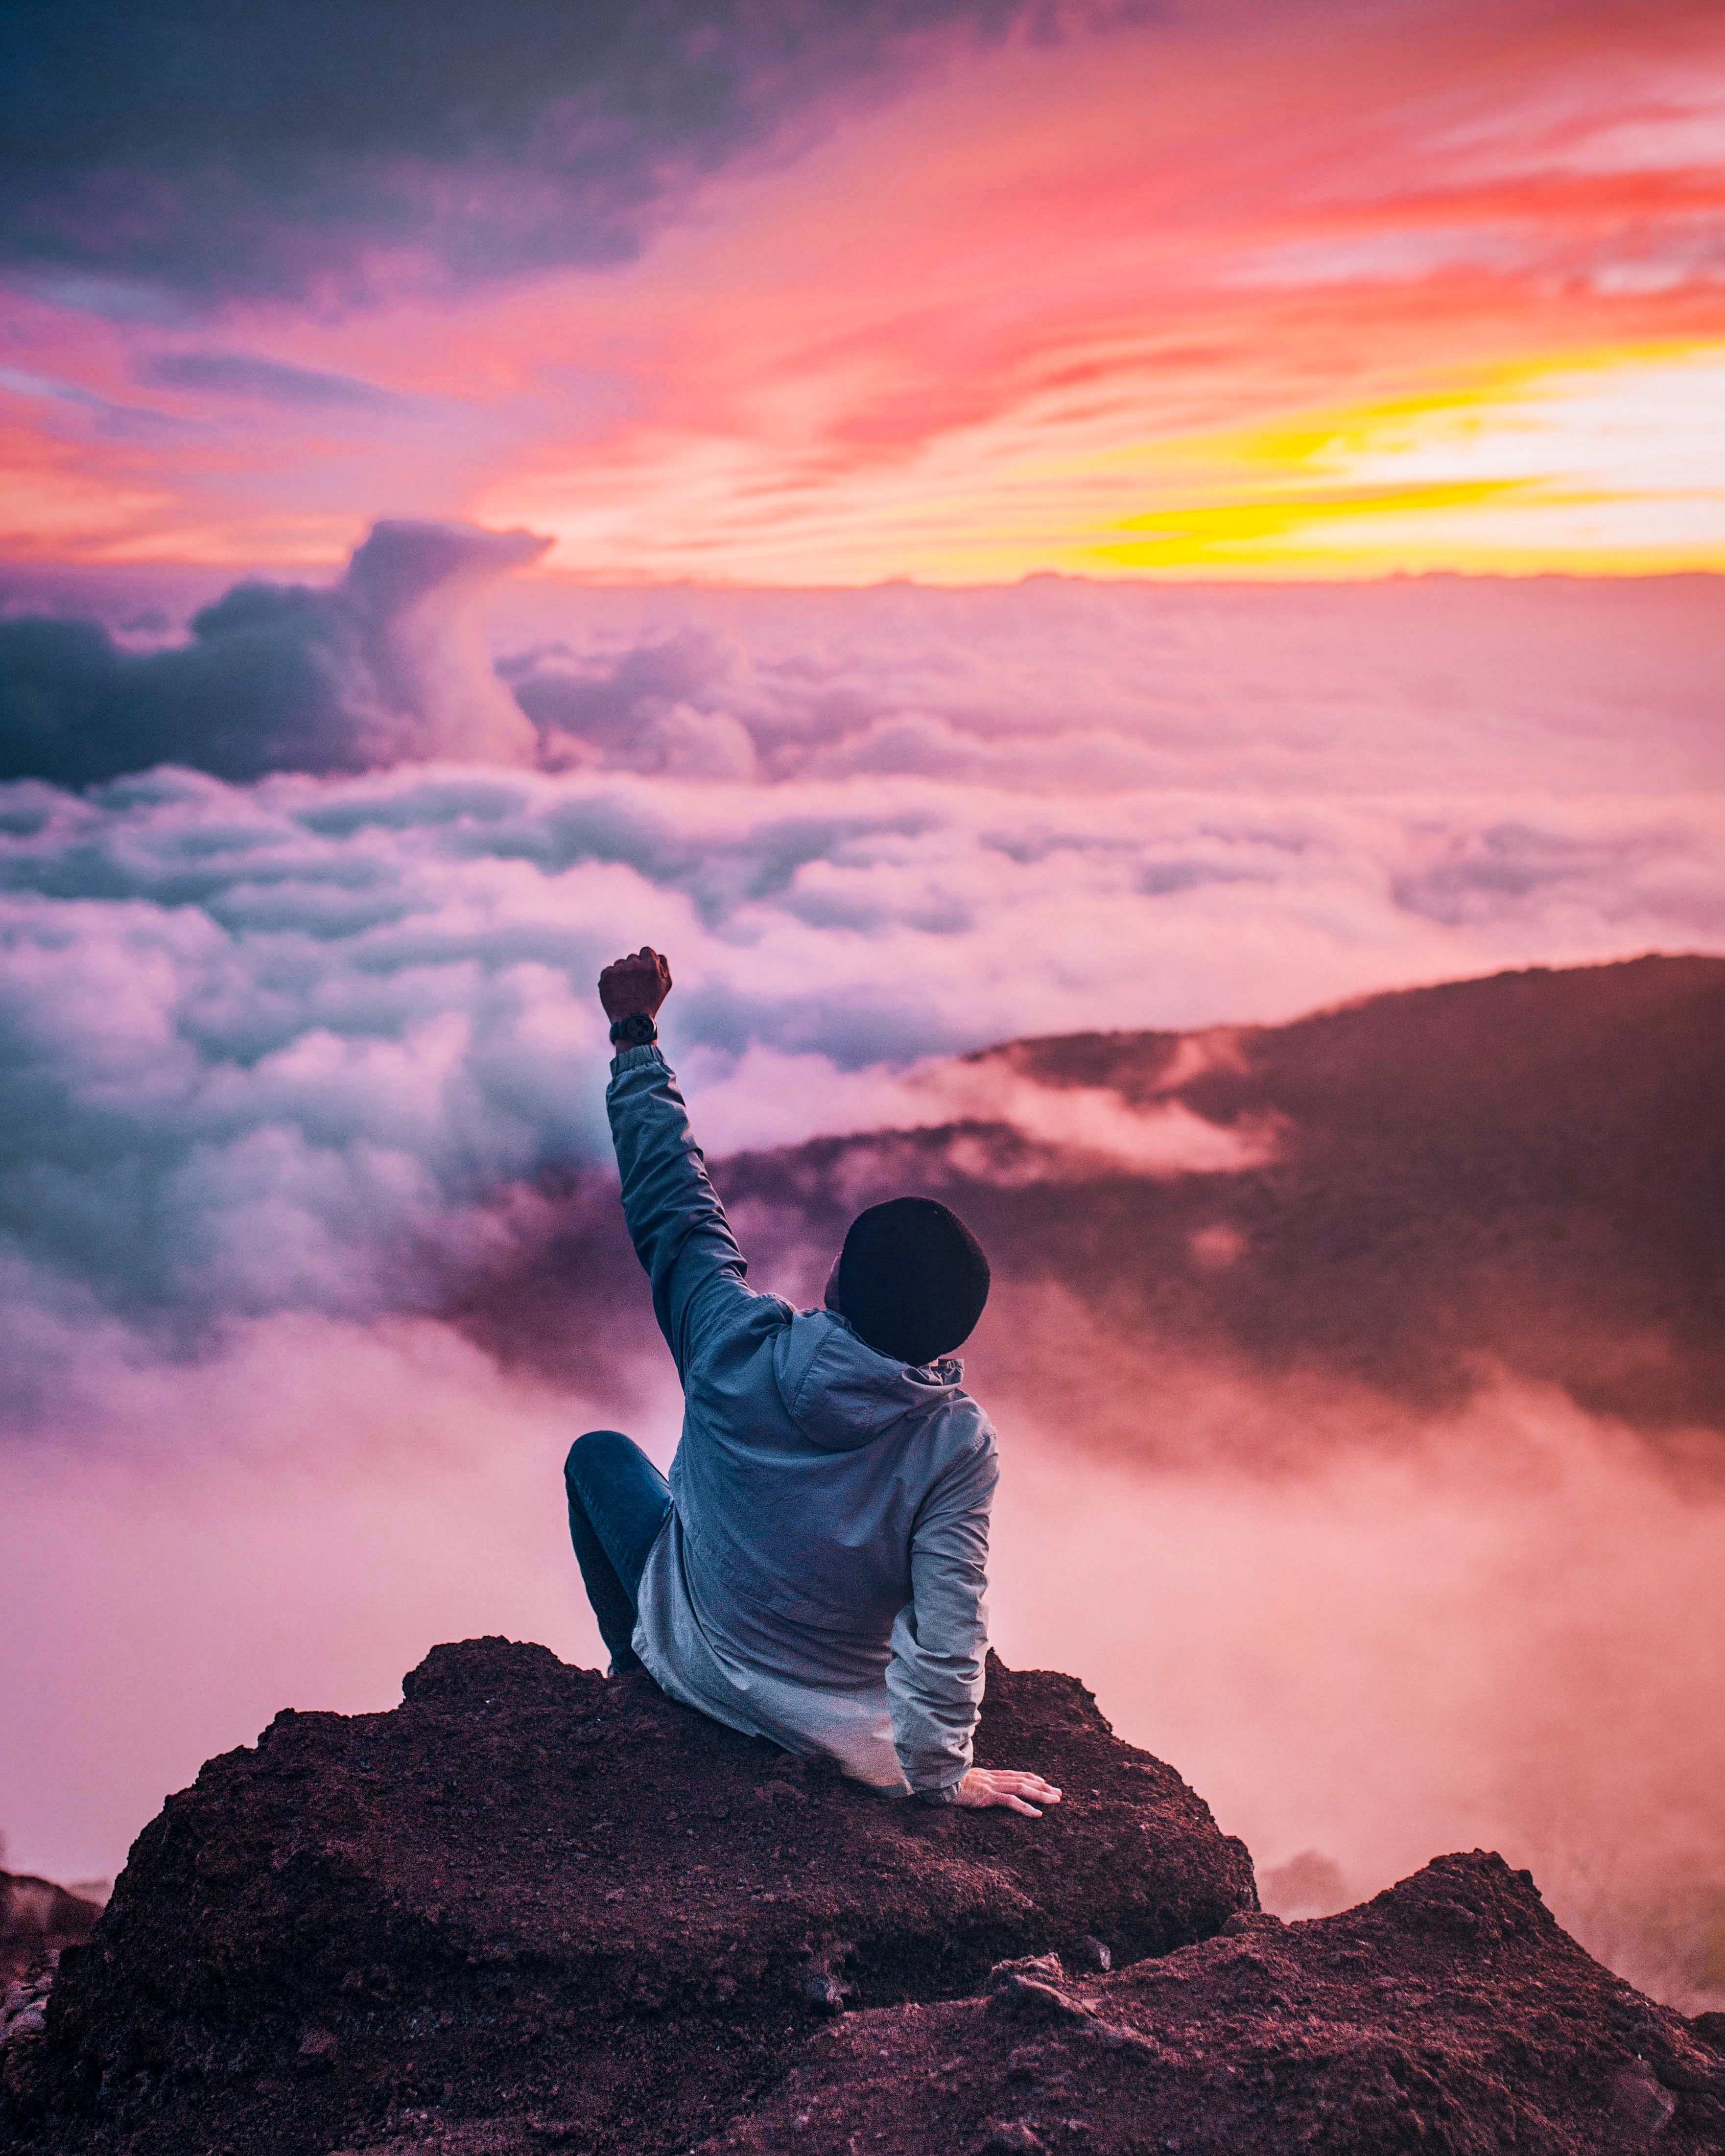
\includegraphics[width=0.9\textwidth]{pictures/final_presentation/achievement.jpg}
				\end{center}
			\end{column}
		\end{columns}
		
	\end{frame}

    % Chapter one "Problem Statement"


    \section{Problem Statement Recap}
    \setbeamertemplate{section page}[BFH-ruled]
    \frame{\sectionpage}
    
    \begin{frame}{Problem Statement Recap "URL-Archiver"}
    	% Kilian
    	\framesubtitle{The ever changing internet}
    	Kilian: \\
    	- Rückblick Project Setup: Erfassung der Ausgangssituation, Themen-Analyse, Stakeholder(-Management), Organisation, Installationen, etc.\\
    	- Eine kurze Repetition der Problemstellung und des Lösungswegs?
    \end{frame}


    \begin{frame}{About what was this project again?}
    	% Kilian
  
    	\begin{columns} % Start the columns environment
    		\begin{column}{0.3\textwidth} % Define the width of the left column
	    		\begin{center}
	    			
\includegraphics[width=0.9\textwidth]{pictures/final_presentation/thinking1.jpg}
	    		\end{center}
    		\end{column}
    	\end{columns}
    \end{frame}

    \begin{frame}{Problem Statement Recap "URL-Archiver"}
    	% Kilian
    	\framesubtitle{The ever changing Internet}
    	\begin{columns} % Start the columns environment
    		\begin{column}{0.7\textwidth} % Define the width of the left column
    			\begin{itemize}
    				\item \textbf{problem statement}
    				\begin{itemize}
                        \item \textbf{ever-changing Internet} (websites are taken down or changed)
    				    \item \textbf{Forensic} (e.g. \textbf{legal report} about a statement on the Internet)
                    \end{itemize}
                    \bigskip
                    \item \textbf{solution}
                    \begin{itemize}
                        \item a java application which \textbf{searches hyperlinks}
                        \item and \textbf{archives} them with an archiving service
                    \end{itemize}
    			\end{itemize}
    		\end{column}
    		\begin{column}{0.3\textwidth} % Define the width of the left column
	    		\begin{center}
	    			
\includegraphics[width=0.9\textwidth]{pictures/final_presentation/idea.jpg}
	    		\end{center}
    		\end{column}
    	\end{columns}
    \end{frame}

    \begin{frame}{Project Goal}
    	% Kilian
    	\begin{columns} % Start the columns environment
    		\begin{column}{0.7\textwidth} % Define the width of the left column
    			\begin{itemize}
    				\item \textbf{Develop a software that\ldots}
    				\begin{itemize}
                        \item \ldots \textbf{searches hyperlinks} within documents
    				    \item \ldots is capable of \textbf{archiving websites}
    				    \item \ldots can \textbf{store} current and archived links in a file
    				    \item \ldots is \textbf{easy} and \textbf{intuitive} to use
                    \end{itemize}
                    
    			\end{itemize}
    		\end{column}
    		\begin{column}{0.3\textwidth} % Define the width of the left column
	    		\begin{center}
	    			
\includegraphics[width=0.9\textwidth]{pictures/final_presentation/goal.jpg}
	    		\end{center}
    		\end{column}
    	\end{columns}
    \end{frame}

    \begin{frame}{Project Setup Review}
    	% Kilian
        \framesubtitle{Initial Situation}
    	\begin{columns} % Start the columns environment
    		\begin{column}{0.7\textwidth} % Define the width of the left column
    			\begin{itemize}
    				\item \textbf{What we knew:}
    				\begin{itemize}
                        \item the end result has to be a \textbf{platform independent java application}
    				    \item we can only use \textbf{FLOSS}-licensed libraries 
    				    \item the software must support \textbf{archive.ph} and \textbf{WayBackMachine}
    				    \item the code must be publicly accessible
                    \end{itemize}
    				
    			\end{itemize}
    		\end{column}
    		\begin{column}{0.3\textwidth} % Define the width of the left column
	    		\begin{center}
	    			\includegraphics[width=0.9\textwidth]{pictures/final_presentation/initial_situation.jpg}
	    		\end{center}
    		\end{column}
    	\end{columns}
    \end{frame}

    \begin{frame}{Project Setup Review}
    	% Kilian
        \framesubtitle{Initial Situation}
    	\begin{columns} % Start the columns environment
    		\begin{column}{0.7\textwidth} % Define the width of the left column
    			\begin{itemize}
    				\item \textbf{What we did first:}
    				\begin{itemize}
                        \item \textbf{project setup}
    				    \item we \textbf{researched} both archiving services and whats possible
    				    \item we designed the rough \textbf{process for user interaction}
    				    \item we decided on a \textbf{software design pattern}
                    \end{itemize}
    				\bigskip
                    \bigskip
                    \bigskip
    			\end{itemize}
    		\end{column}
    		\begin{column}{0.23\textwidth} % Define the width of the left column
	    		\begin{center}
	    			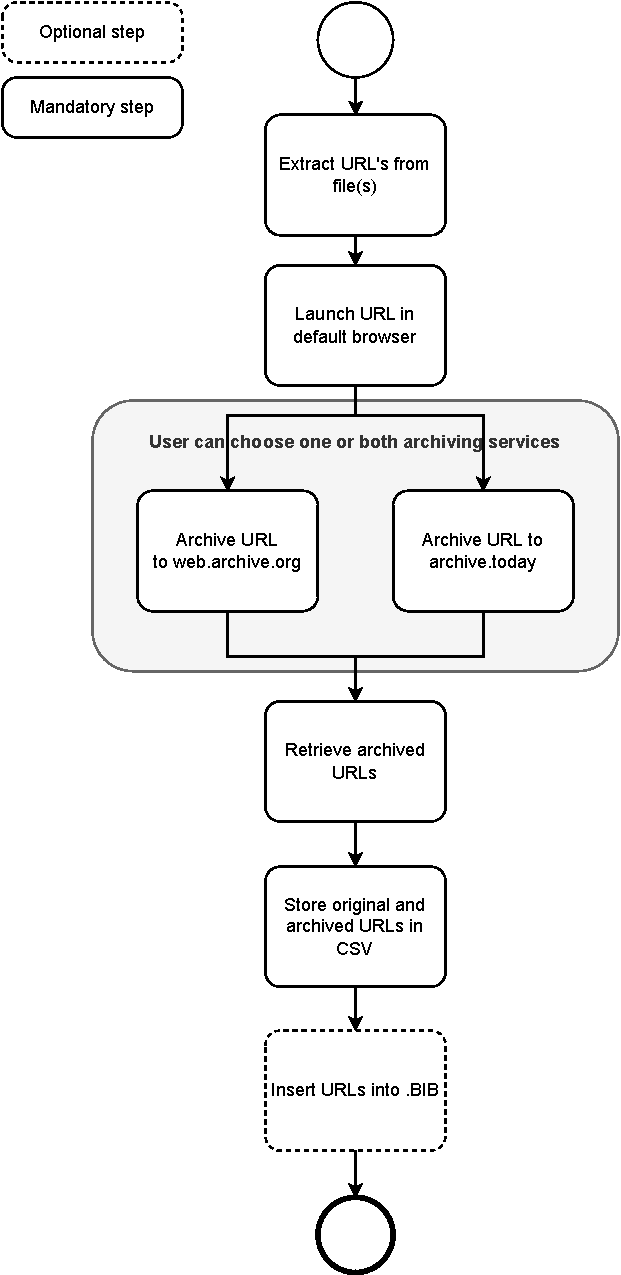
\includegraphics[width=0.9\textwidth]{figures/process_model-simple-vertikal}
	    		\end{center}
    		\end{column}
    	\end{columns}
    \end{frame}

    \begin{frame}{Project Setup Review}
    	% Kilian
        \framesubtitle{Installation / Project Setup}
    	\begin{columns} % Start the columns environment
    		\begin{column}{0.7\textwidth} % Define the width of the left column
    			\begin{itemize}
    				\item creation of a new \textbf{github repository} for public accessibility
    				\item setting up a \textbf{jira project} (with epics and first stories)
    				\item installing the \textbf{latest java version}
    			\end{itemize}
    		\end{column}
    		\begin{column}{0.23\textwidth} % Define the width of the left column
	    		\begin{center}
	    			
\includegraphics[width=0.5\textwidth]{pictures/github-mark.png}
                    
\includegraphics[width=0.9\textwidth]{pictures/jira_logo.png}
                    
\includegraphics[width=0.9\textwidth]{pictures/Java-Logo.png}
	    		\end{center}
    		\end{column}
    	\end{columns}
    \end{frame}



	\section{Solution Overview}
	% Nicolin
	\setbeamertemplate{section page}[BFH-ruled]
	\frame{\sectionpage}
	
	\begin{frame}{Project Requirements}
		% Nicolin
		\framesubtitle{Requirements met}
		\begin{columns} % Start the columns environment
			\begin{column}{0.7\textwidth} % Define the width of the left column
				\begin{itemize}
					\item[\checkmark] Accepts \textbf{directories}, \textbf{Unicode text} (.BIB, .TEX, .HTML, etc.), or \textbf{.PDF files} as input.
					\item[\checkmark] Extracts \textbf{all URLs} from the files.
					\item[\checkmark] Can \textbf{open} URLs in a web browser.
					\item[\checkmark] Can \textbf{archive URLs} to \textbf{archive.today} and \textbf{the Wayback Machine}.
					\item[\checkmark] Retrieves archived URLs.
					\item[\checkmark] \textbf{Outputs a CSV file} with key-value pairs of original and archived URLs.
					\item[\checkmark] Can \textbf{add archived URLs to a .BIB file}.
					\item[(\checkmark)] The program code should be \textbf{minimal, modular, and self-explaining}.
				\end{itemize}
				
			\end{column}
			\begin{column}{0.3\textwidth} % Define the width of the left column
				\begin{center}
					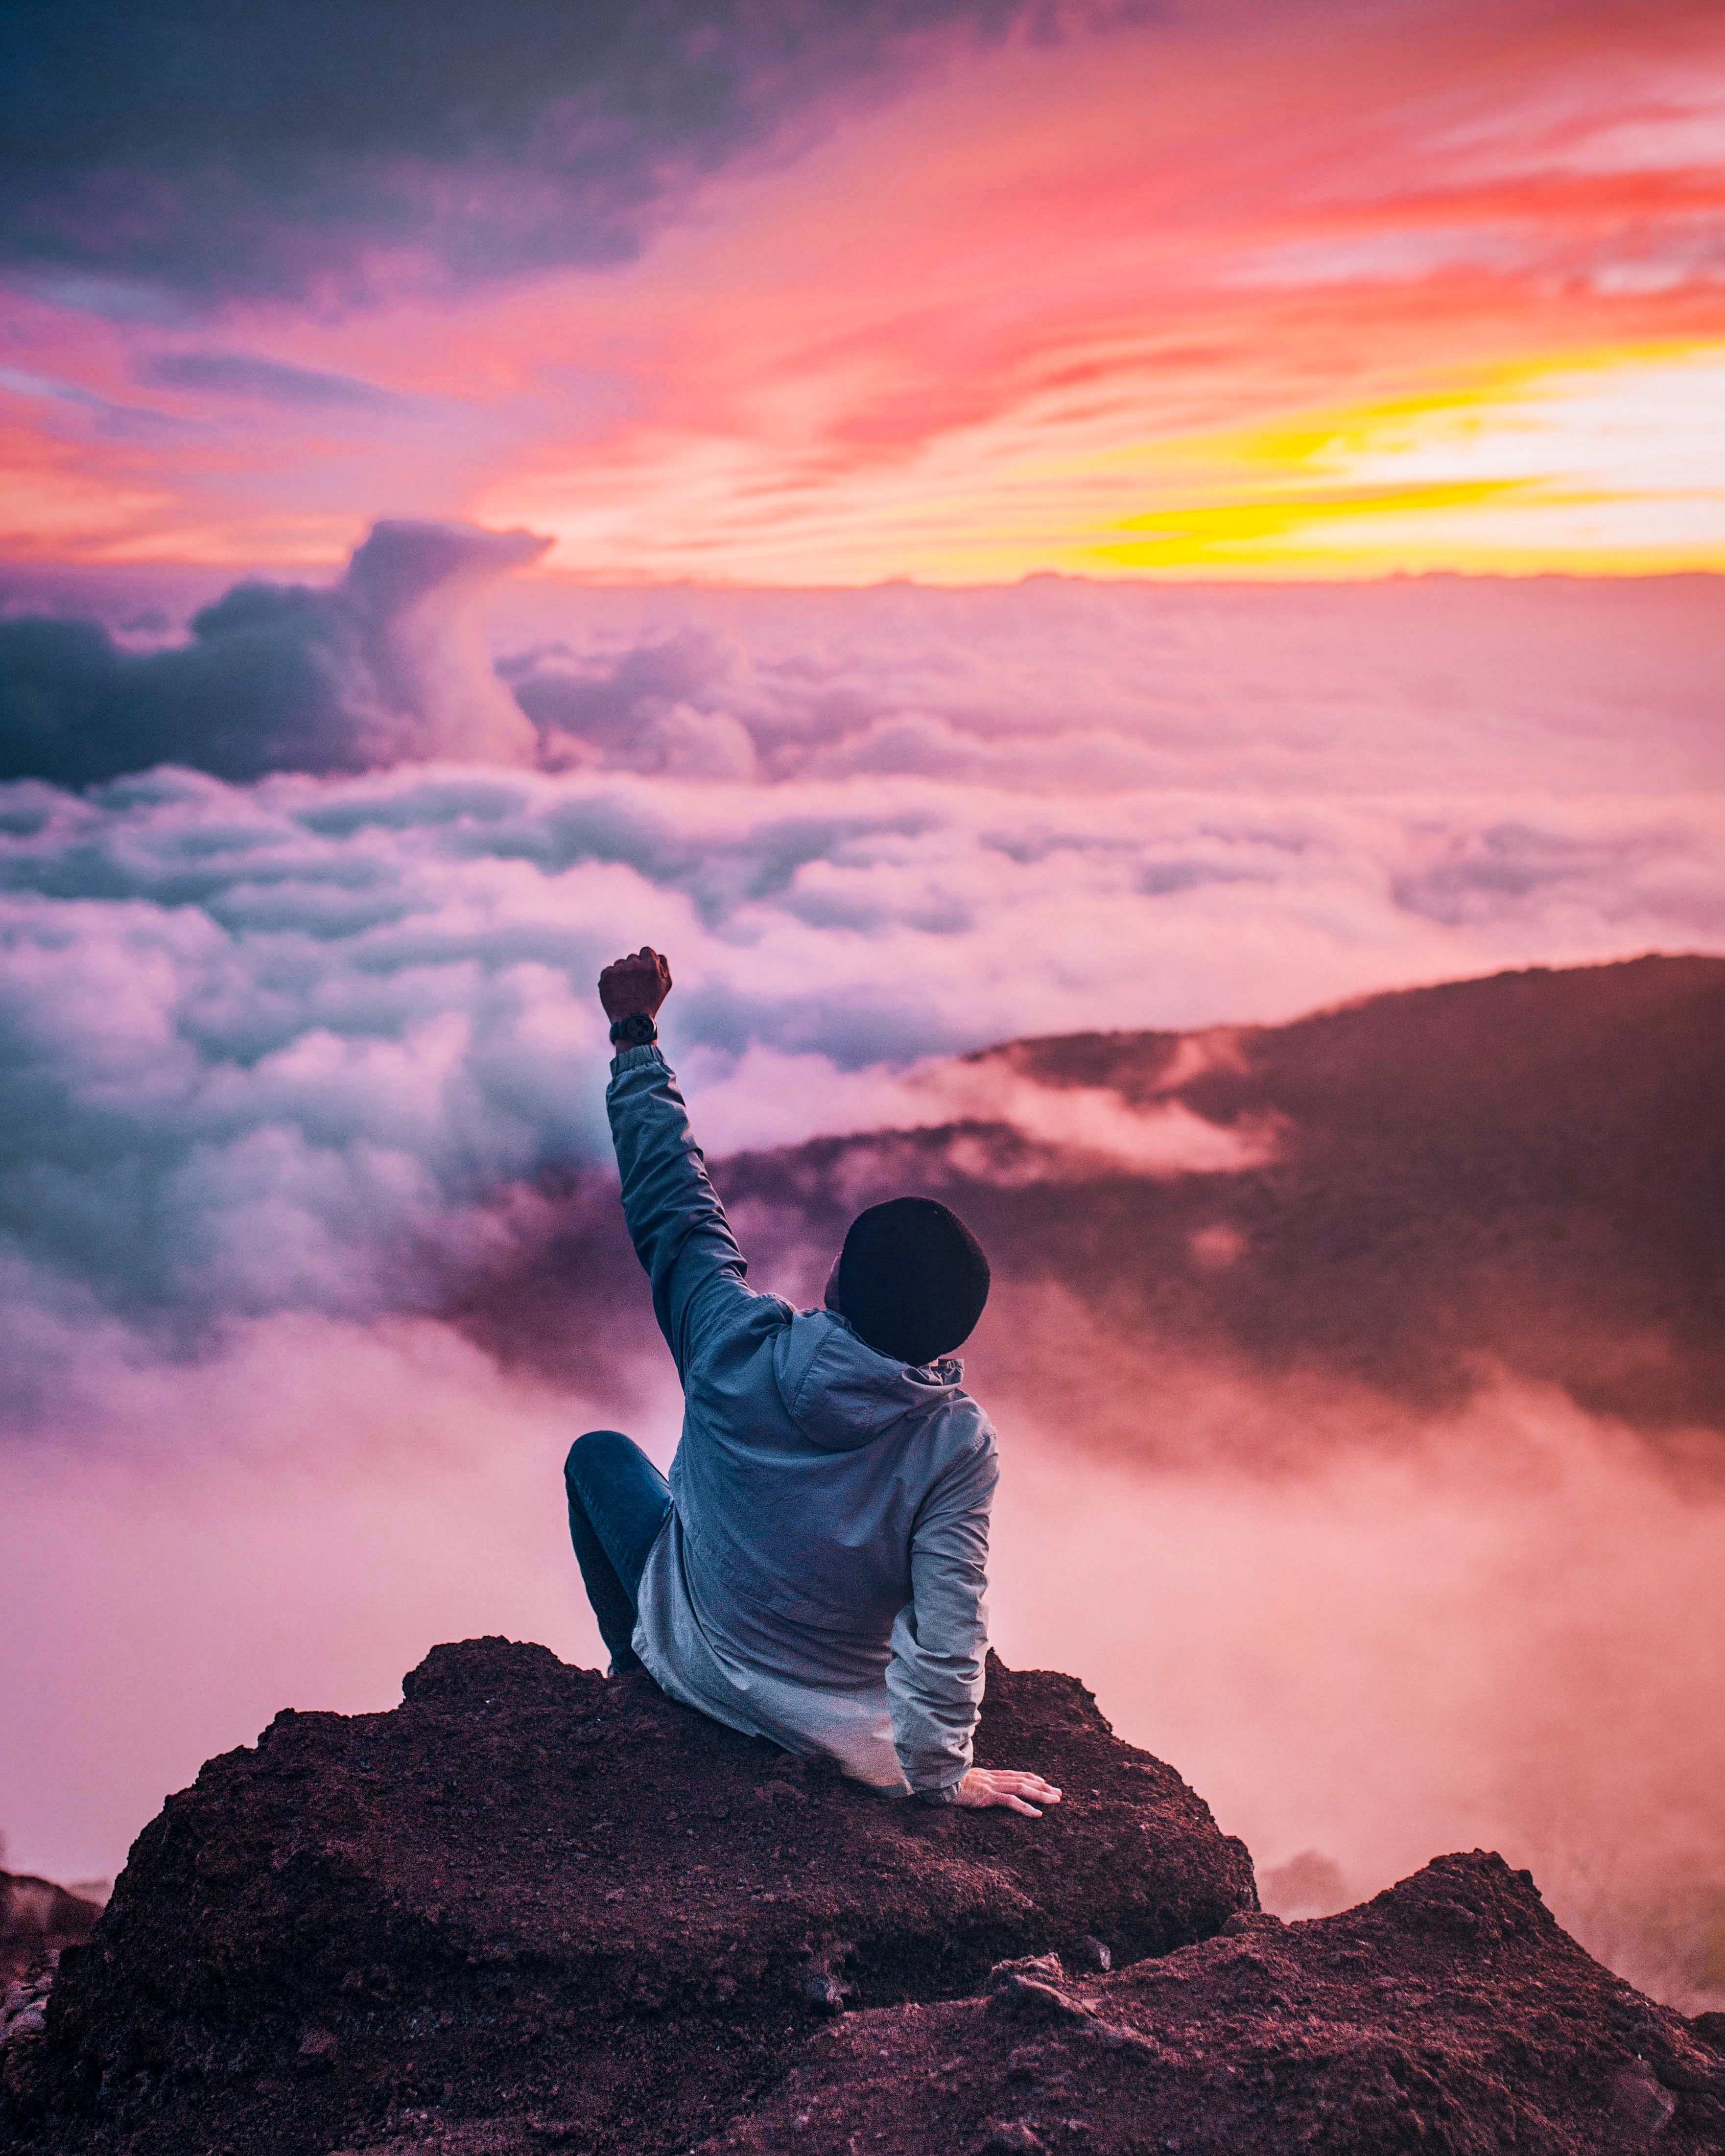
\includegraphics[width=0.9\textwidth]{pictures/final_presentation/achievement.jpg}
				\end{center}
			\end{column}
		\end{columns}
		\note[item]{Thank you Kilian and welcome from my side too.}
		\note[item]{I will now explain our application to you in more detail. }
		\note[item]{Firstly, the project requirements. Our application should be able to read directories with Unicode text or PDF files. Of course, it should also be possible to read individual files. The application should then read all URLs from the files. The user should then be able to open the URLs in their browser and archive the URLs to the two services archive.today and the Wayback Machine. Of course, our application should get back the archived version and save it. When all URLs have been processed, the user can save the URLs in a CSV file or, if possible, back into a Bibtex file.}
		\note[item]{Last but not least, the code should be minimal, modular and self-explanatory. }
		\note[item]{We have fulfilled all these requirements. However, our supervisor has the last word on the last one in particular. }
		
	\end{frame}
	
	\subsection{Process Model}
	\begin{frame}{Process Model}
		\framesubtitle{Workflow for URL Extraction and Archiving}
		\begin{itemize}
			\item User can \textbf{skip URLs}, \textbf{launch them}, \textbf{access help} or \textbf{quit} the program at \textbf{any time}
		\end{itemize}
		\vspace{0.8cm}
		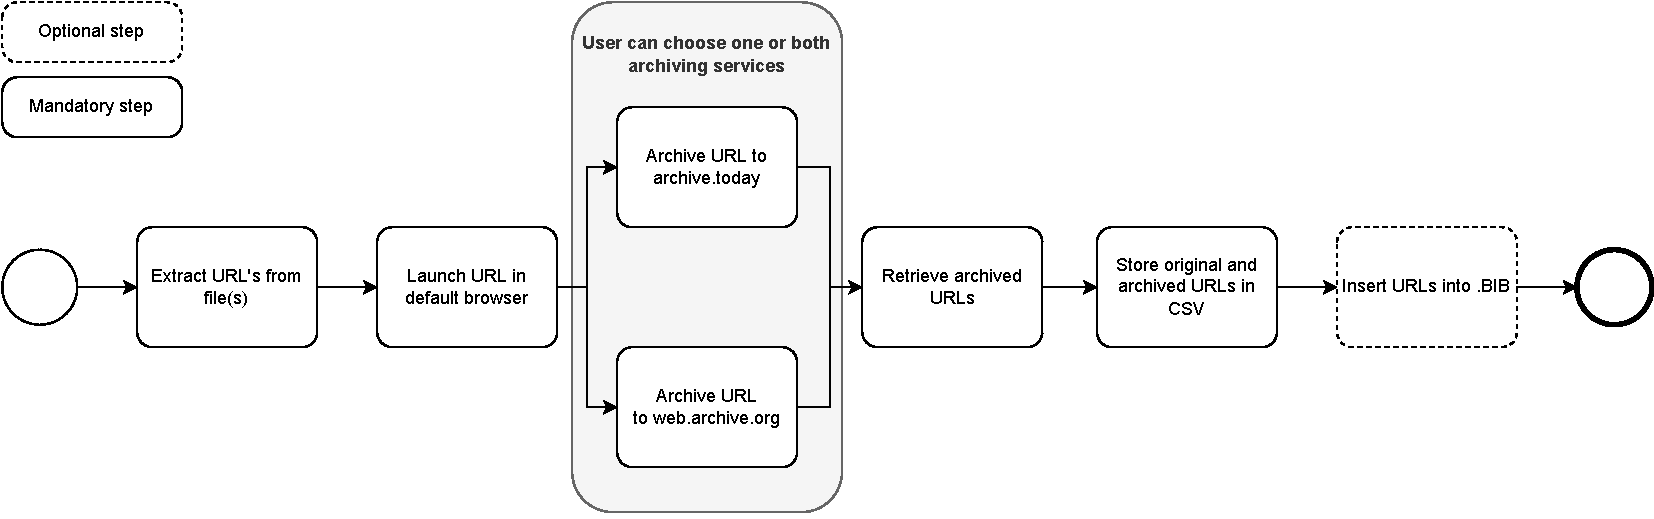
\includegraphics[width=1\textwidth]{pictures/process_model-simple}
		\note[item]{Now that I've talked about the what, let's move on to the how. }
		\note[item]{You know this slide from the intermediate presentation, it shows the main path that a user takes in our application. This gives a good overview of our application. }
		\note[item]{The user gives the URL archiver a path, the URLs are extracted and the user can open them in his default browser.}
		\note[item]{The user can then archive the URL with one or both of the archiving services. }
		\note[item]{The application receives the archived version and finally saves it to a CSV file or writes it back to a Bibtex file. }
	\end{frame}
    
    
    \begin{frame}{Command line application}
    	% Nicolin
    	\framesubtitle{Why a command line and not a GUI application?}
    	\begin{columns} % Start the columns environment
    		\begin{column}{0.7\textwidth} % Define the width of the left column
    			\begin{itemize}
    				\item \textbf{Focus on Logic:} Emphasis on functional depth over visual design.
    				\item \textbf{Technical Audience:} Suited for users proficient in command-line environments.
    				\item \textbf{Efficiency in Development:} Streamlines the development process by focusing less on UI design.
    				\item \textbf{Flexibility and Scalability:} Provides a stable base for future feature expansion.
    				\item \textbf{Foundation for Future Enhancements:} The MVC pattern lays the groundwork for easy GUI integration later.
    			\end{itemize}
    		\end{column}
    		\begin{column}{0.3\textwidth} % Define the width of the left column
	    		\begin{center}
	    			
\includegraphics[width=0.9\textwidth]{pictures/final_presentation/cmd_vs_gui.png}
	    		\end{center}
    		\end{column}
    	\end{columns}
    	\note[item]{We have decided in favour of a command line program and against a GUI. For various reasons.}
    	\note[item]{On the one hand, because we could focus on the logic and didn't have to build a responsive GUI.}
    	\note[item]{ On the other hand, our stakeholders are in the technical world and should therefore have few problems with a CLI application. }
    	\note[item]{With a CLI application we create a stable basis to build on. }
    	\note[item]{With the MVC pattern we can add a GUI in the future with little effort. }
    	
    \end{frame}

	\begin{frame}{Architecture}
		\framesubtitle{Employing the \textbf{MVC} Pattern}
		
		\begin{columns} % Start the columns environment
			\begin{column}{0.5\textwidth} % Define the width of the left column
				\begin{itemize}
					\item Modular design for \textbf{easy extension}
					\item Separate data, view, and control flow
					\item Facilitates the potential \textbf{addition of a GUI}
				\end{itemize}
			\end{column}
			
			\begin{column}{0.5\textwidth} % Define the width of the right column
				\begin{center}
					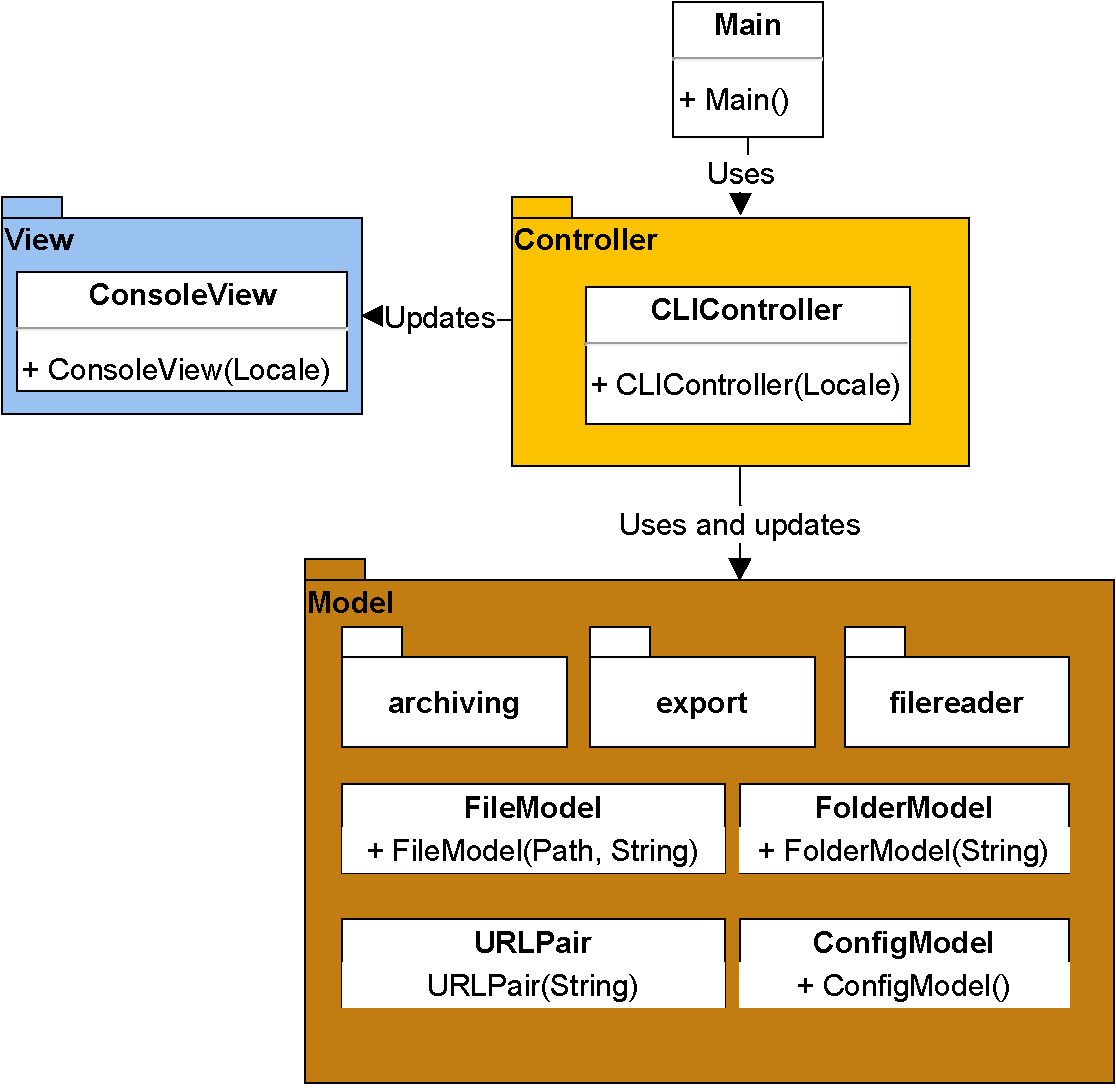
\includegraphics[width=0.9\textwidth]{pictures/final_presentation/mvc_diagram-Highlevel_MV_Presentation.pdf}
				\end{center}
			\end{column}
		\end{columns} % End the columns environment
		\note[item]{Speaking of the MVC pattern. As already mentioned, this pattern allows us to easily extend the application in the future. }
		\note[item]{As the view is separated from the model by the controller. }
		\note[item]{This means that these parts can be easily exchanged without having to make major changes to the others. }
	\end{frame}

	\begin{frame}{Architecture}
		\framesubtitle{Factory Pattern}
		\begin{columns} % Start the columns environment
			\begin{column}{0.6\textwidth} % Define the width of the left column
				\begin{itemize}
					\item \textbf{Archiving Services Integration:} Factory Pattern streamlines incorporating various web archiving services.
					\item \textbf{Selenium Web Drivers:} Facilitates easy swapping or addition of drivers for different browsers.
					\item \textbf{CSV and Bibtex Exporting:} Simplifies the process of exporting data in different file formats.
					\item \textbf{File Reader Flexibility:} Allows seamless integration and extension of file reading capabilities.
					\item \textbf{Ease of Extension:} The Factory Pattern enables straightforward expansion and customization of functionalities.
				\end{itemize}
			\end{column}
			\begin{column}{0.4\textwidth} % Define the width of the right column
				\begin{center}
					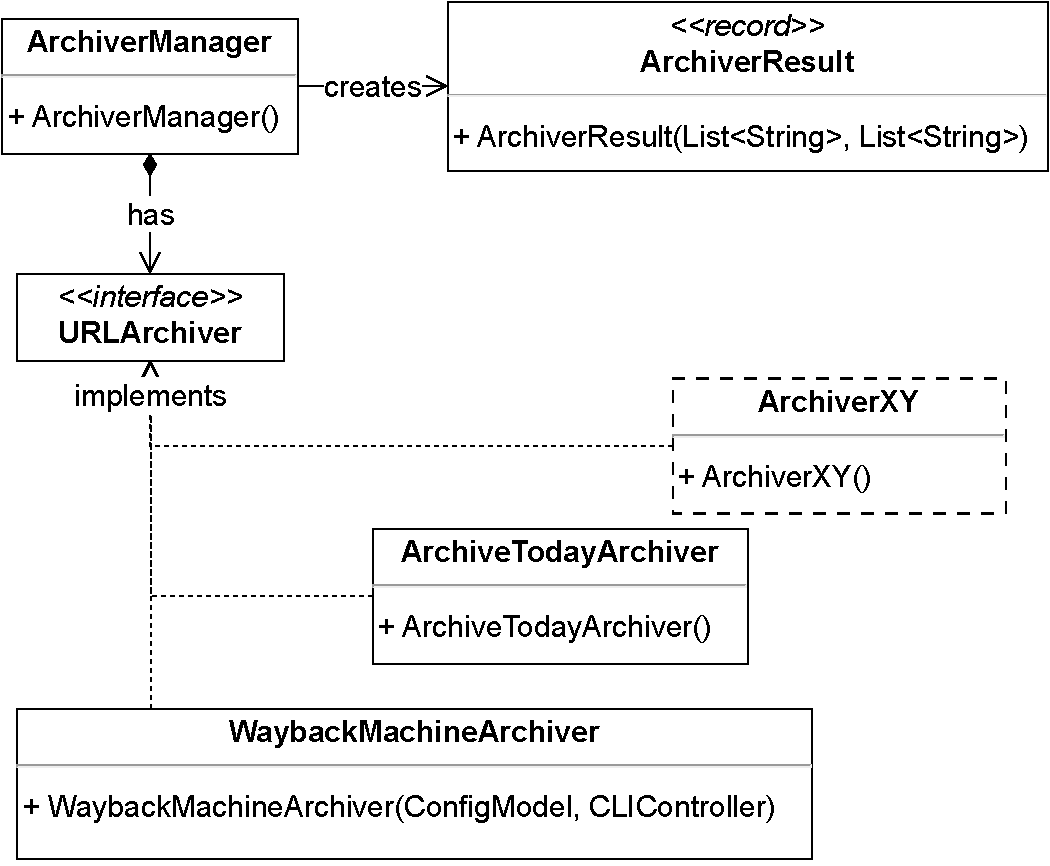
\includegraphics[width=0.8\textwidth]{pictures/final_presentation/URL_Archiver_Class_Diagram-ArchiverManager.pdf}
				\end{center}
			\end{column}
		\end{columns} % End the columns environment
		\note[item]{We have also used the factory pattern where appropriate. }
		\note[item]{Specifically with the archiving services, the Selenium web drivers, when exporting to a CVS and Bibtex file and when reading the files. }
		\note[item]{As you can see on the right, using the archiving services as an example, this allows us a simple extension. }
	\end{frame}

	\begin{frame}{Enhancing Functionality and Flexibility}
		\framesubtitle{Configuration, Internationalization, and Testing}
		\begin{columns} % Start the columns environment
			\begin{column}{0.6\textwidth} % Define the width of the left column
				\begin{itemize}
					\item \textbf{Configuration File Usage:} Preserves settings between program sessions.
					\begin{itemize}
						\item \textbf{Stored Settings:} Includes Wayback Machine API keys and default browser.
					\end{itemize}
					\item \textbf{i18n Implementation:} Lays groundwork for multilingual support.
					\item \textbf{Unit Testing:} Comprehensive tests written for all relevant classes.
				\end{itemize}
			\end{column}
			\begin{column}{0.4\textwidth} % Define the width of the right column
				\begin{center}
					
\includegraphics[width=0.7\textwidth]{pictures/final_presentation/unit_international_config.png}
				\end{center}
			\end{column}
		\end{columns} % End the columns environment
		\note[item]{We have also made various decisions to improve the functionality and flexibility of the application. }
		\note[item]{We save configurations in a configuration file. }
		\note[item]{We have laid the foundation for multilingualism... }
		\note[item]{... and are testing all relevant classes with unit tests; there are currently 107 unit tests in total. }
	\end{frame}

	\begin{frame}{Ease of Use: Installation Simplified}
		\framesubtitle{Custom Scripts for Cross-Platform Compatibility}
		\begin{columns} % Start the columns environment
			\begin{column}{0.6\textwidth} % Define the width of the left column
				\begin{itemize}
					\item \textbf{Simplified Compilation and Installation:} Tailored scripts for Windows, Linux, and macOS.
					\item \textbf{User-Friendly Scripts:} Enable straightforward application compilation and execution.
					\item \textbf{Flexible Installation Options:} Users can choose to compile then run, or do both in one step.
				\end{itemize}
			\end{column}
			\begin{column}{0.4\textwidth} % Define the width of the right column
				\begin{center}
					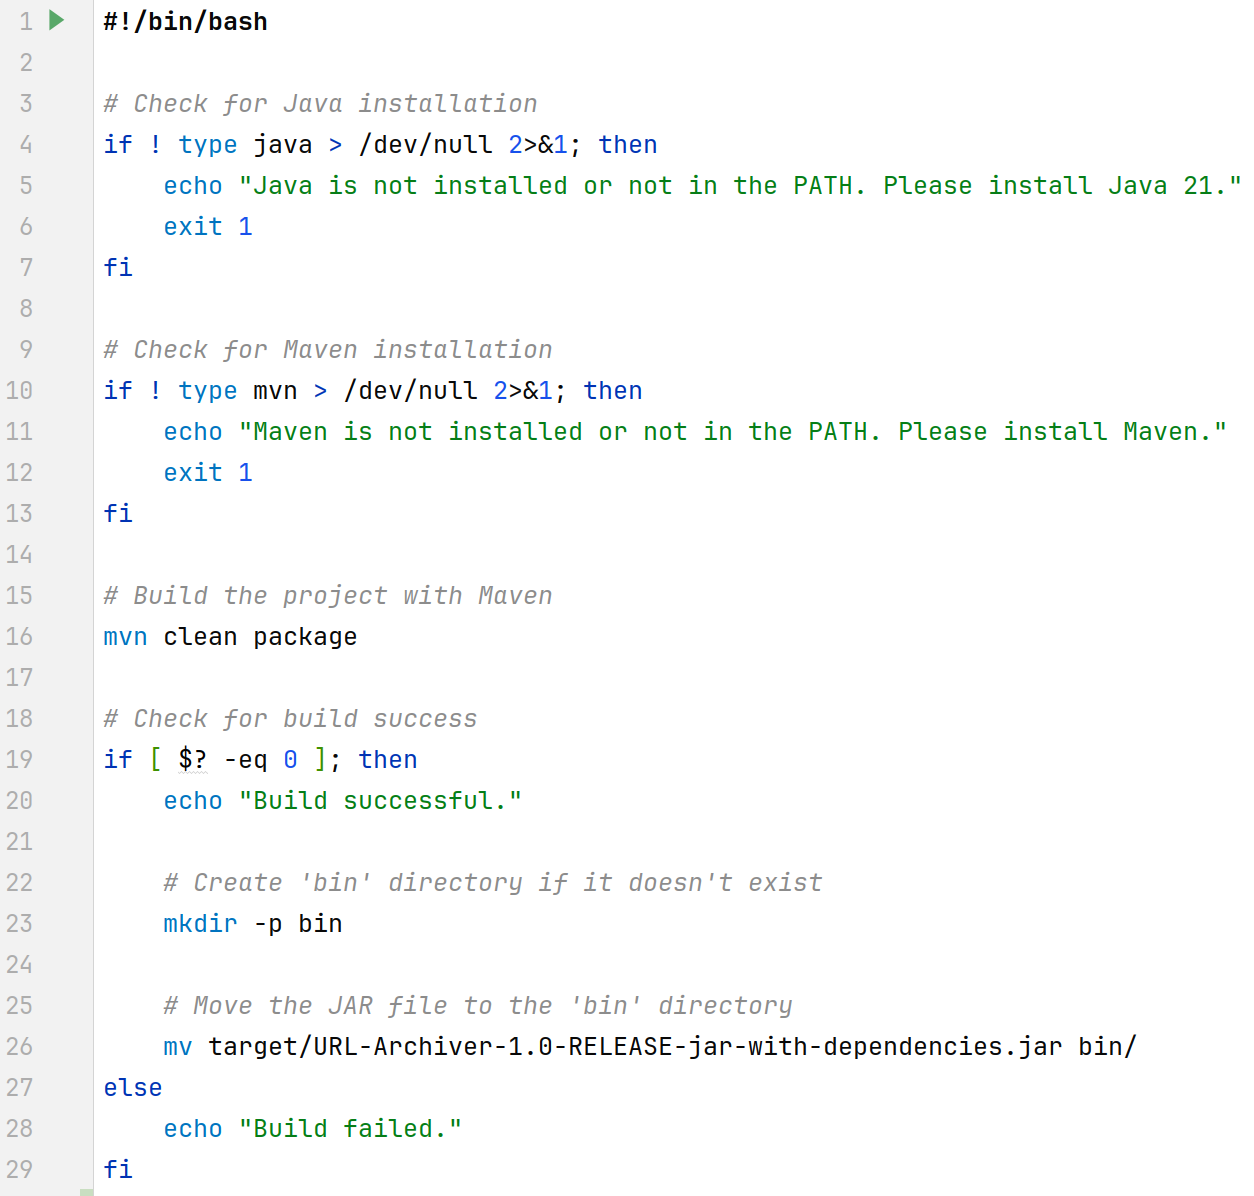
\includegraphics[width=0.9\textwidth]{pictures/final_presentation/build_script.png}
				\end{center}
			\end{column}
		\end{columns} % End the columns environment
		\note[item]{To make it as easy as possible for users to get started with the application, we have created compilation and run scripts. }
		\note[item]{Of course bash scripts for Linux and macOS and PowerShell scripts for Windows. }
	\end{frame}

	\section{Live-Demo}
	% Nicolin
	\setbeamertemplate{section page}[BFH-ruled]
	\frame{\sectionpage}


	\begin{frame}{Implementation Details}
		% Nicolin
		\framesubtitle{}
	\end{frame}


	\begin{frame}{Demonstration of the Solution}
		% Nicolin
		\framesubtitle{}
	\end{frame}

	\begin{frame}{SCRUM}
		% Abidin
		\framesubtitle{}
	\end{frame}

    \section{Conclusion}
	% Kilian
	\setbeamertemplate{section page}[BFH-ruled]
	\frame{\sectionpage}

    \begin{frame}{Conclusion: Project Goal}
        \begin{columns} % Start the columns environment
            \begin{column}{0.5\textwidth} % Define the width of the left column
                \begin{itemize}
                    \item[\checkmark] \textbf{Develop a software that}\ldots
                    \begin{itemize}
                        \item[\checkmark] \ldots \textbf{searches hyperlinks} within documents
                        \item[\checkmark] \ldots is capable of \textbf{archiving websites}
                        \item[\checkmark] \ldots can \textbf{store} current and archived links in a file
                        \item[\checkmark] \ldots is \textbf{easy} and \textbf{intuitive} to use
                    \end{itemize}
                \end{itemize}
            \end{column}
            \begin{column}{0.3\textwidth} % Define the width of the left column
                \begin{center}
                    
\includegraphics[width=0.6\textwidth]{pictures/sherlock}
                \end{center}
            \end{column}
        \end{columns}
    \end{frame}

    \begin{frame}{Future Work}
        \framesubtitle{What can be done to improve the application further}
        \begin{columns} % Start the columns environment
            \begin{column}{0.5\textwidth} % Define the width of the left column
                \begin{itemize}
                    \item Add more \textbf{archiving services} (such as Memento Time Travel)
                    \item Support more \textbf{input file types} (e.g. .docx)
                    \item Integrate a \textbf{graphical interface}
                    \item Implement \textbf{multilingual} support
                \end{itemize}
            \end{column}
            \begin{column}{0.3\textwidth} % Define the width of the left column
                \begin{center}
                    
\includegraphics[width=1\textwidth]{pictures/final_presentation/Business_team_2.jpg}
                \end{center}
            \end{column}
        \end{columns}
    \end{frame}

    \begin{frame}{Lessons learned}
        \framesubtitle{Team}
        \begin{columns} % Start the columns environment
            \begin{column}{0.5\textwidth} % Define the width of the left column
                \begin{itemize}
                    \item \textbf{Basic code structure}
                    \item \textbf{Code Reviews} more often 
                    \item \textbf{Weeklys} are important
                \end{itemize}
            \end{column}
            \begin{column}{0.3\textwidth} % Define the width of the left column
                \begin{center}
                    
\includegraphics[width=1\textwidth]{pictures/Learnings}
                \end{center}
            \end{column}
        \end{columns}
    \end{frame}

    \begin{frame}{Lessons learned (personal)}
        \framesubtitle{Kilian Wampfler}
        \begin{columns} % Start the columns environment
            \begin{column}{0.5\textwidth} % Define the width of the left column
                \begin{itemize}
                    \item good refresher for java development
                    \item the team worked well together
                    \item my junit tests could be improved (consistency & quality)
                    \item my git commit messages according to convention
                \end{itemize}
            \end{column}
            \begin{column}{0.3\textwidth} % Define the width of the left column
                \begin{center}
                    \hexagonimage{pictures/wampfler_2}
                \end{center}
            \end{column}
        \end{columns}
    \end{frame}


    \begin{frame}{Lessons learned (personal)}
        \framesubtitle{Nicolin Dora}
        \begin{columns} % Start the columns environment
            \begin{column}{0.5\textwidth} % Define the width of the left column
                \begin{itemize}
                    \item 
                \end{itemize}
            \end{column}
            \begin{column}{0.3\textwidth} % Define the width of the left column
                \begin{center}
                    \hexagonimage{pictures/dora_2.png}
                \end{center}
            \end{column}
        \end{columns}
    \end{frame}

    \begin{frame}{Lessons learned (personal)}
        \framesubtitle{Abidin Vejseli}
        \begin{columns} % Start the columns environment
            \begin{column}{0.5\textwidth} % Define the width of the left column
                \begin{itemize}
                    \item 
                \end{itemize}
            \end{column}
            \begin{column}{0.3\textwidth} % Define the width of the left column
                \begin{center}
                    \hexagonimage{pictures/vejseli_2.png}
                \end{center}
            \end{column}
        \end{columns}
    \end{frame}

    \section{Questions?}
    \setbeamertemplate{section page}[BFH-ruled]
    \frame{\sectionpage}


%---------------------------------------------------------------------------------------%
%																						%
%						Slides from intermediate presentation							%	
%																						%
%---------------------------------------------------------------------------------------%

    \begin{frame}{Problem Statement Recap "URL-Archiver"}
    	% Kilian
        \framesubtitle{The ever changing internet}
        \begin{columns} % Start the columns environment
            \begin{column}{0.6\textwidth} % Define the width of the left column
                \begin{itemize}
                    \item \textbf{ever-changing internet} (websites are taken down or changed)
                    \item not a problem for everyday internet users but\ldots
                    \item \ldots what about \textbf{documents} (e. g. theses, documentations etc.)
                    \begin{itemize}
                        \item invalid links to content-relevant information
                        \item invalid quote links
                        \item old documents may contain numerous broken hyperlinks
                    \end{itemize}
                    \item another case: \textbf{Forensic}
                    \begin{itemize}
                        \item e.g. \textbf{legal report} about a statement on the Internet
                    \end{itemize}
                \end{itemize}
            \end{column}
            \begin{column}{0.3\textwidth} % Define the width of the left column
                \begin{center}
                    
\includegraphics[width=0.6\textwidth]{pictures/broken_link}
                \end{center}
            \end{column}
        \end{columns}
    \end{frame}

	
	

    \begin{frame}{Problem Statement}
        \framesubtitle{Simple Solution}
        \begin{columns} % Start the columns environment
            \begin{column}{0.5\textwidth} % Define the width of the left column
                \begin{itemize}
                    \item Archive the \textbf{actual state} of the linked websites
                    \begin{itemize}
                        \item Wayback machine
                        \item archive.today
                        \item Memento Time Travel
                        \item and more…
                    \end{itemize}
                    \item But who has the \textbf{time} and \textbf{motivation}?
                    \begin{itemize}
                        \item \ldots to search each hyperlink
                        \item \ldots to manually archive each website
                    \end{itemize}
                \end{itemize}
            \end{column}
            \begin{column}{0.4\textwidth} % Define the width of the left column
                \begin{center}
                    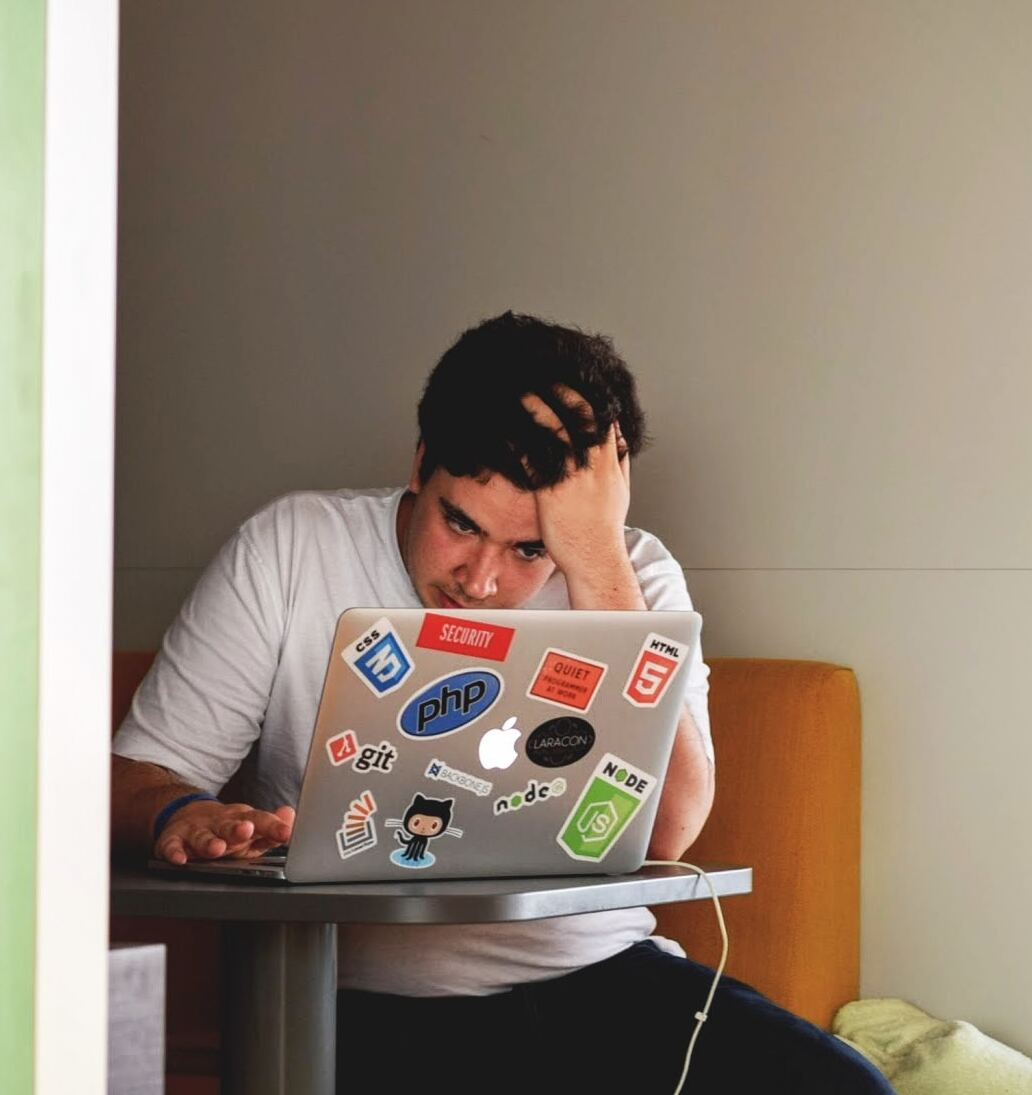
\includegraphics[width=0.7\textwidth]{pictures/frustrated}
                \end{center}
            \end{column}
        \end{columns}
    \end{frame}

    \subsection{Project Goal}
    \begin{frame}{Project Goal}
        \begin{columns} % Start the columns environment
            \begin{column}{0.5\textwidth} % Define the width of the left column
                \begin{itemize}
                    \item \textbf{Develop a software that}\ldots
                    \begin{itemize}
                        \item \ldots \textbf{searches hyperlinks} within documents
                        \item \ldots is capable of \textbf{archiving websites}
                        \item \ldots can \textbf{store} current and archived links in a file
                        \item \ldots is \textbf{easy} and \textbf{intuitive} to use
                    \end{itemize}
                \end{itemize}
            \end{column}
            \begin{column}{0.3\textwidth} % Define the width of the left column
                \begin{center}
                    
\includegraphics[width=0.6\textwidth]{pictures/sherlock}
                \end{center}
            \end{column}
        \end{columns}
    \end{frame}

    \subsection{Requirements}
    \begin{frame}{Functional Requirements}
        \begin{columns} % Start the columns environment
            \begin{column}{0.5\textwidth} % Define the width of the left column
                \begin{itemize}
                    \item \textbf{The software must be}\ldots
                    \begin{itemize}
                        \item \ldots a \textbf{Java application} that is compatible with multiple platforms
                        \item \ldots Free and Open Source Software licensed \textbf{(FLOSS)}
                        \item \ldots capable of archiving websites on \textbf{archive.ph} or/and \textbf{WayBackMachine}
                        \item \ldots capable of generating a \textbf{CSV-file} with key-value (URL, archived URL)
                    \end{itemize}
                \end{itemize}
            \end{column}
            \begin{column}{0.3\textwidth} % Define the width of the left column
                \begin{center}
                    
\includegraphics[height=1cm]{pictures/Java-Logo}
                    \vspace{1em}
                    
\includegraphics[height=1cm]{pictures/Wayback_Machine_logo}
                    \vspace{1em}
                    
\includegraphics[height=1cm]{pictures/archive_today_logo}
                \end{center}
            \end{column}
        \end{columns}


    \end{frame}

    \begin{frame}{Non-Functional requirement}
        \begin{columns} % Start the columns environment
            \begin{column}{0.5\textwidth} % Define the width of the left column
                \begin{itemize}
                    \item Coding Norm
                    \item publicly accessible
                    \item Project-Method: \textbf{SCRUM}
                    \item public documents in English
                    \item project report with \textbf{LaTeX}
                    %\item The program code should be minimal, modular, and self-explaining
                    %\item The program code should be published in a git repository
                    %\item The project must be carried out according to scrum
                    %\item Public documents should be written in English
                    %\item LaTeX should be used for the project report
                \end{itemize}
            \end{column}
            \begin{column}{0.4\textwidth} % Define the width of the left column
                \begin{center}
                    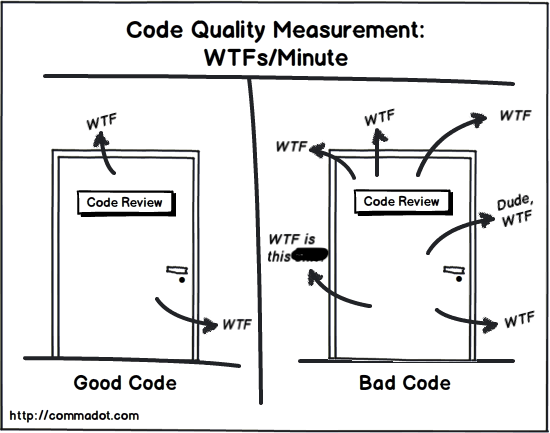
\includegraphics[width=0.8\textwidth]{pictures/clean-code-1}
                \end{center}
            \end{column}
        \end{columns}
    \end{frame}
%-------------------------------%

% Chapter two "Solving the Problem"


    \section{Solving The Problem}
    \setbeamertemplate{section page}[BFH-ruled]
    \frame{\sectionpage}

    \subsection{Process Model}
    \begin{frame}{Process Model}
        \framesubtitle{Workflow for URL Extraction and Archiving}
        \begin{itemize}
            \item User can \textbf{skip URLs}, \textbf{launch them}, \textbf{access help} or \textbf{quit} the program at \textbf{any time}
        \end{itemize}
        \vspace{0.8cm}
        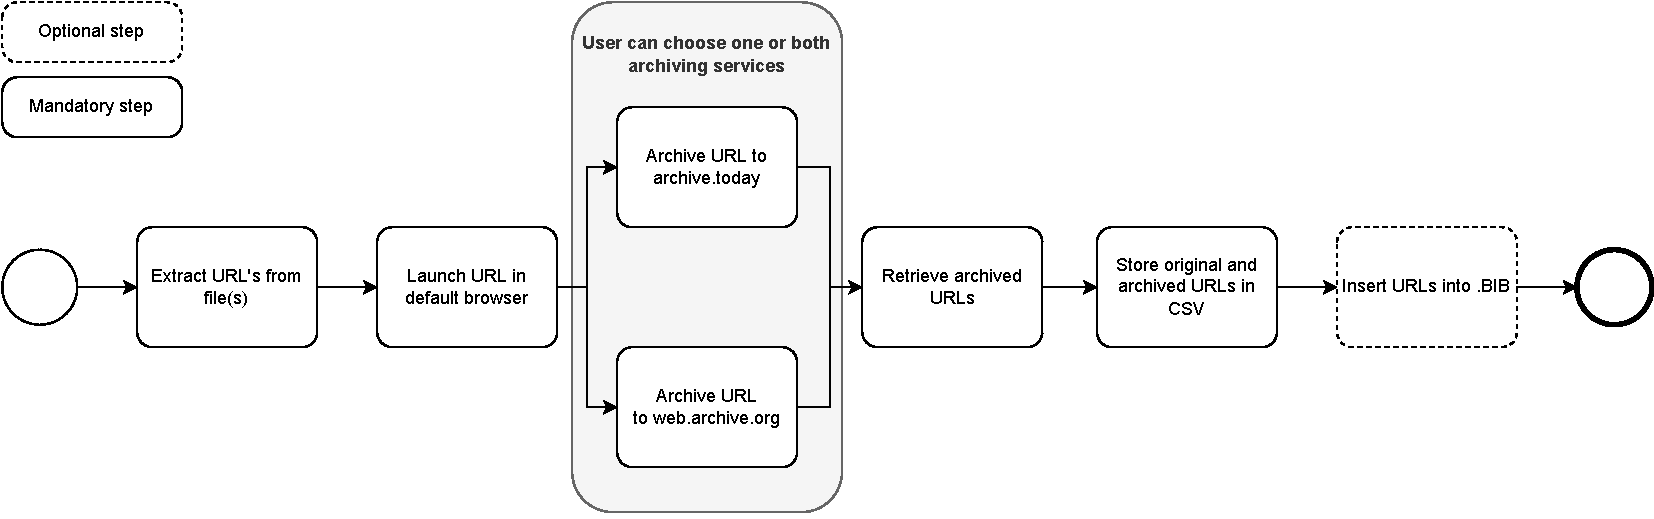
\includegraphics[width=1\textwidth]{pictures/process_model-simple}
        \note[item]{Thank you for coming from my side too.}
        \note[item]{First lets talk about how an user can archive urls. }
        \note[item]{----------------------------------------------------------}
        \note[item]{For this you can see here a rough overview of how a user navigates through the application to archive URLs. }
        \note[item]{The user can open the current URL in their default browser, access the help section, or view the archived URLs at any time.}
        \note[item]{The user does not need to archive a url, he can skip the archiving process.}
        \note[item]{Now to the more technical part.}
    \end{frame}

    \subsection{Architecture}
    \begin{frame}{High Level Class Diagram}
        \framesubtitle{Overview}
        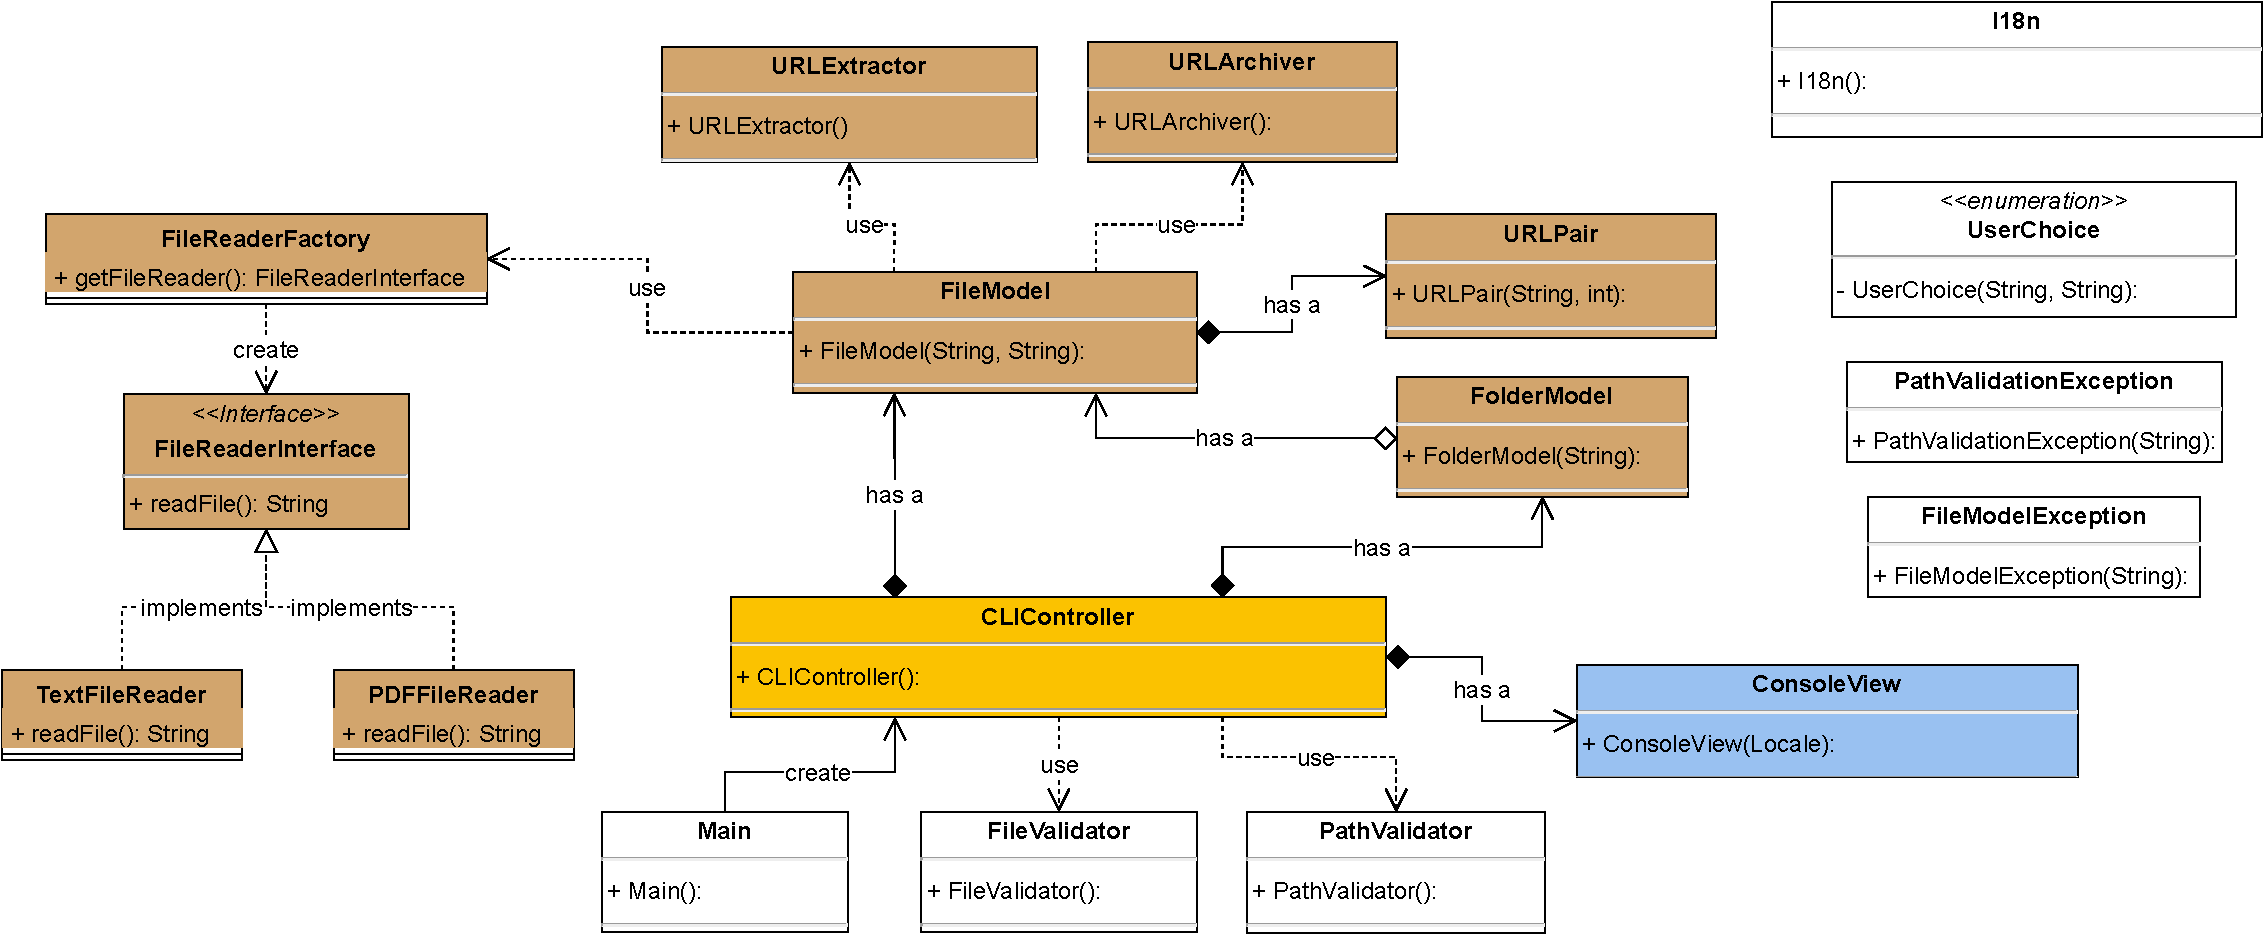
\includegraphics[width=1\textwidth]{figures/URL_Archiver_Class_Diagram-Presentation_0}
        \note[item]{To demonstrate how we meet the requirements for our application, which Kilian presented earlier, I will now provide a high-level overview of our structure and its individual components.}
        \note[item]{It is important to note that this is our current structure, subject to expansion and adaptation as the project advances. }
        \note[item]{The Main class serves as the application's entry point.}
        \note[item]{CLIController interprets user commands, validates paths and types, and selects the data model.}
        \note[item]{FileModel manages individual file data, and stores URL associations.}
        \note[item]{FolderModel deals with file groupings within folders, integrating multiple FileModel instances.}
        \note[item]{URLPair links original to the archived URL. }
        \note[item]{I18n enables the application to support multiple languages, enhancing global usability.}
        \note[item]{UserChoice defines possible user actions with corresponding i18n keys, aiding in international user interaction.}
        \note[item]{ConsoleView acts as the communication hub, utilizing UserChoice for navigation and i18n for language support.}
        \note[item]{Now I would like to discuss some aspects of the architecture in greater detail. }
    \end{frame}

    \begin{frame}{Architecture}
        \framesubtitle{Employing the \textbf{MVC} Pattern}

        \begin{columns} % Start the columns environment
            \begin{column}{0.5\textwidth} % Define the width of the left column
                \begin{itemize}
                    \item Modular design for \textbf{easy extension}
                    \item Separate data, view, and control flow
                    \item Facilitates the potential \textbf{addition of a GUI}
                \end{itemize}
            \end{column}

            \begin{column}{0.5\textwidth} % Define the width of the right column
                \begin{center}
                    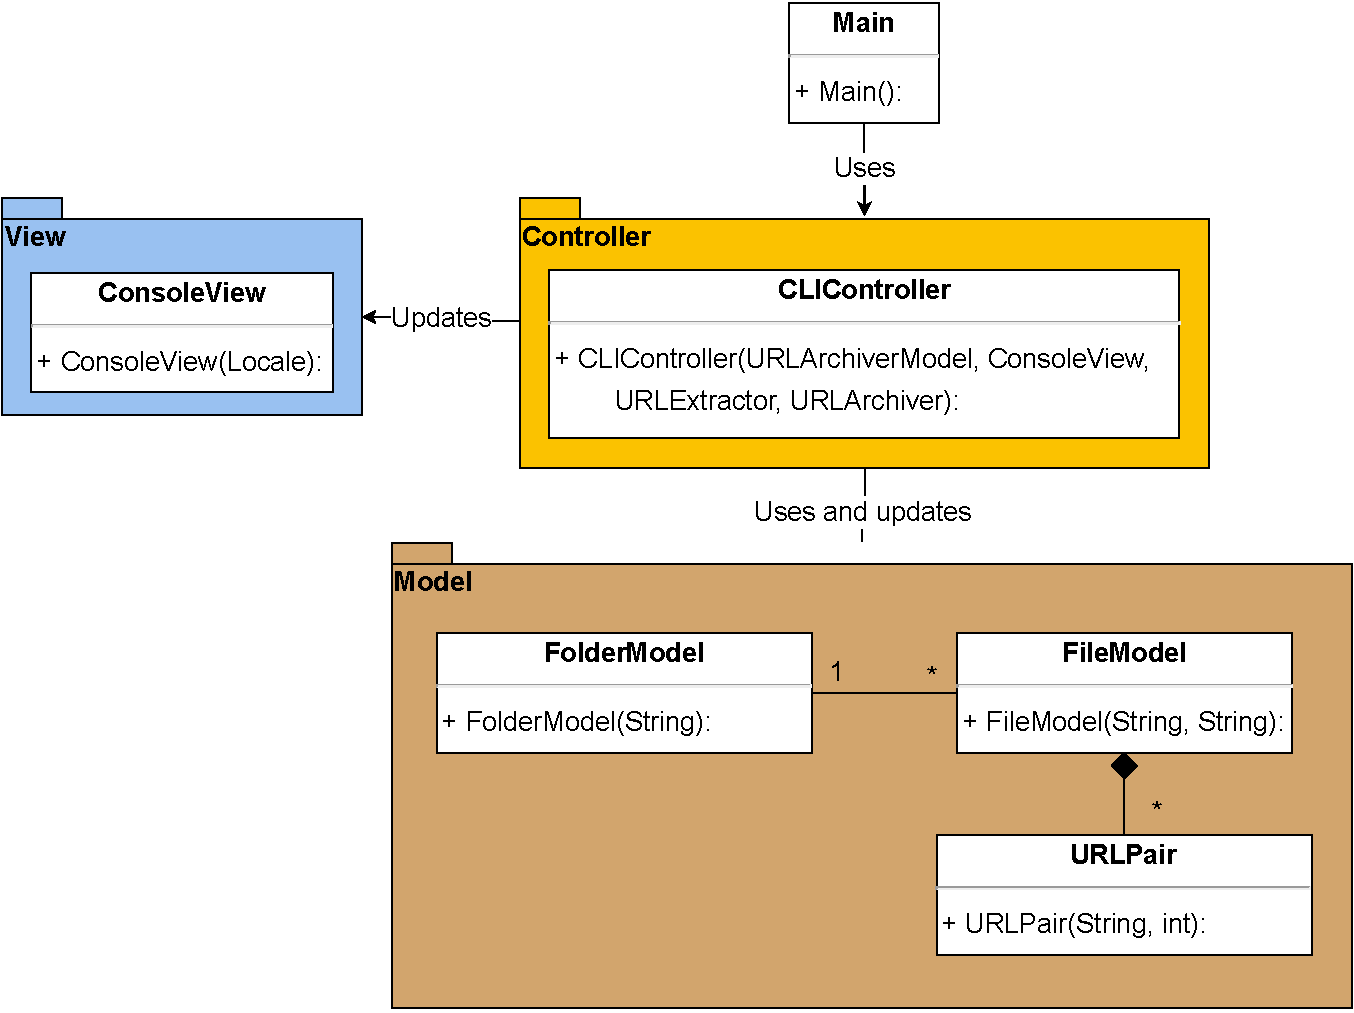
\includegraphics[width=1\textwidth]{figures/mvc_diagram-Detailed_MVC}
                \end{center}
            \end{column}
        \end{columns} % End the columns environment
        \note[item]{As you may have observed, we utilize the MVC pattern, among other techniques, to ensure the scalability of the application.  }
        \note[item]{This involves separating the business logic from the presentation using a controller. }
        \note[item]{This enables us to easly switch out the Command Line Interface with a Graphical User Interface.}
        \note[item]{But that's not all!}
    \end{frame}

%\begin{frame}{High Level Class Diagram}
%    \framesubtitle{Main}
%    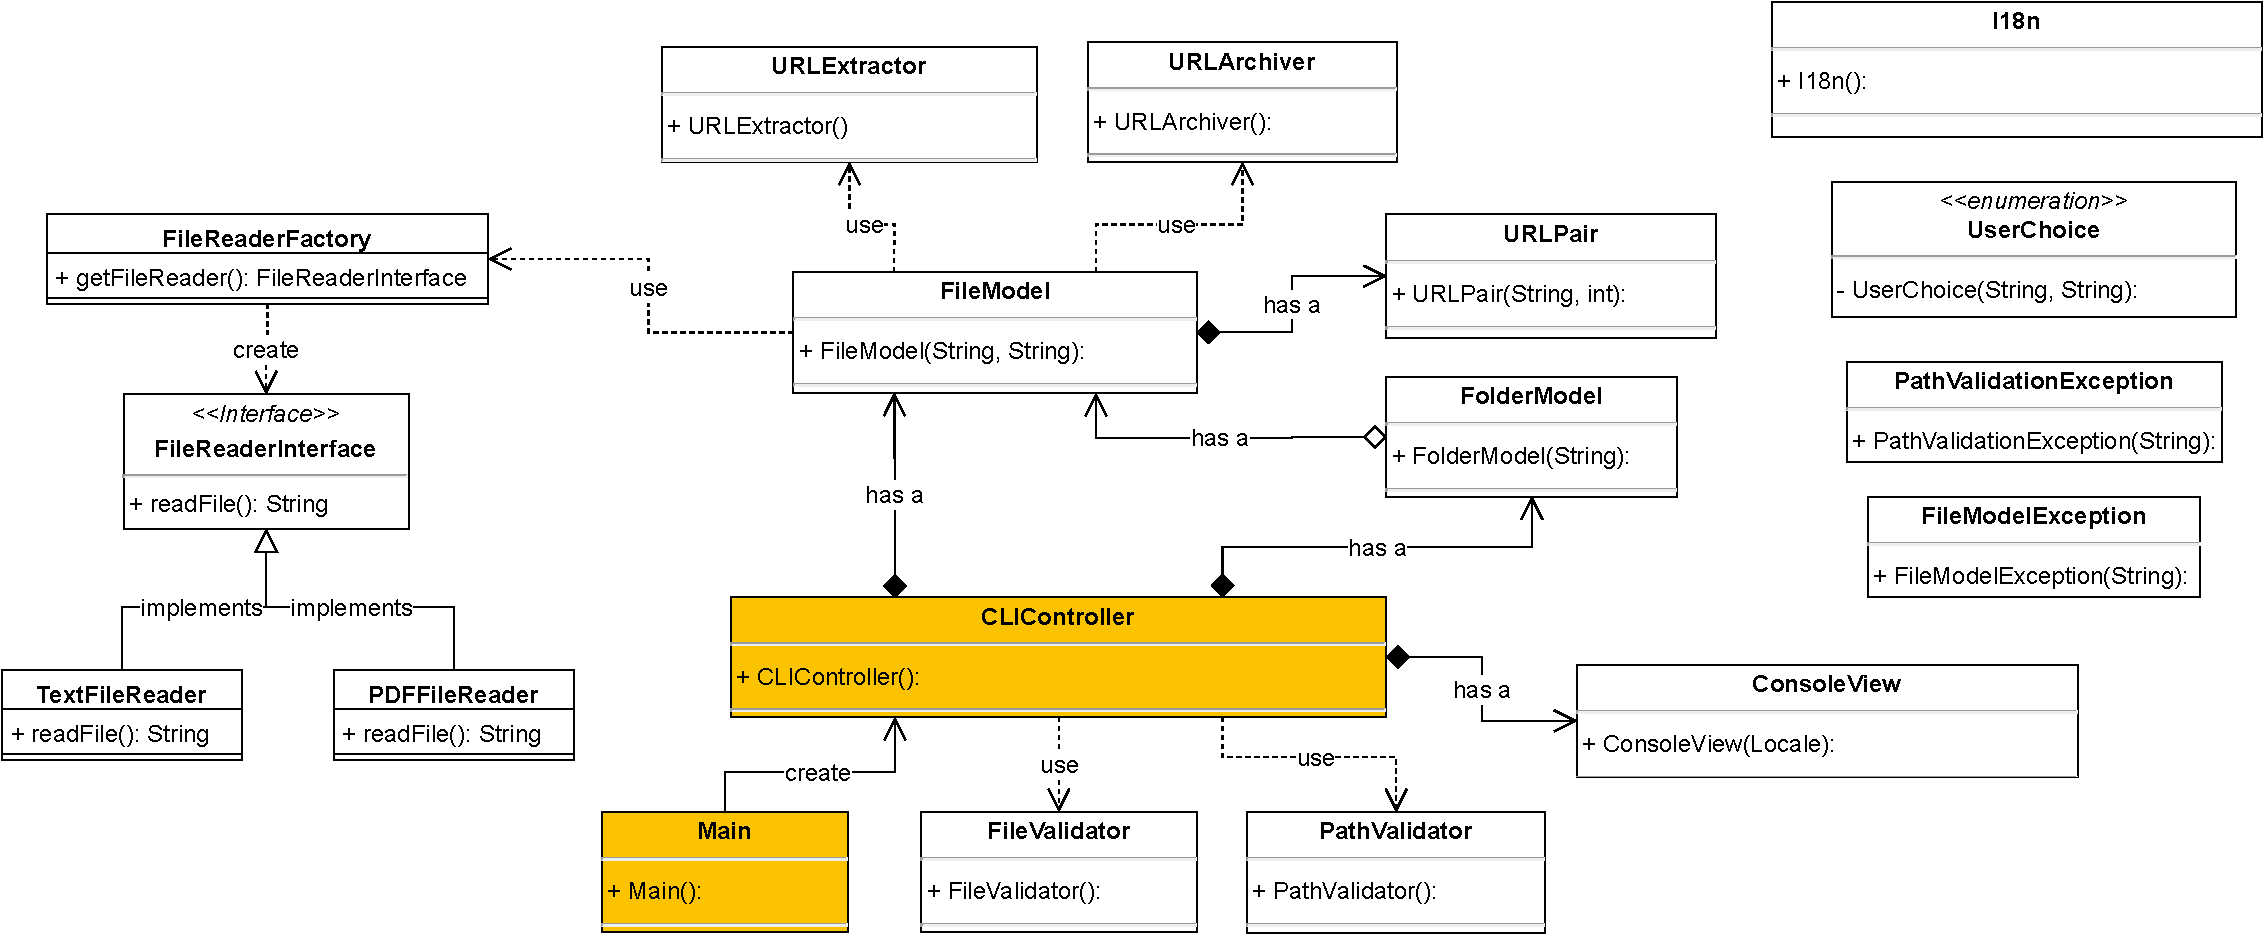
\includegraphics[width=1\textwidth]{pictures/URL_Archiver_Class_Diagram-Presentation_1}
%    \note[item]{I know you're thinking: didn't he say high level?}
%    \note[item]{I know, I know, but I'll walk you through the diagram with the orange markers. }
%    \note[item]{So just focus on the orange and stay with me.  }
%    \note[item]{----------------------------------------------------------}
%    \note[item]{As usual, the Main class starts the program. }
%    \note[item]{It directly initializes the controller class. }
%    \note[item]{The Controller class is the control instance of the entire application. It connects the business logic with the command line interface. Keyword MVC pattern.}
%\end{frame}
%
%\begin{frame}{High Level Class Diagram}
%    \framesubtitle{CLIController}
%    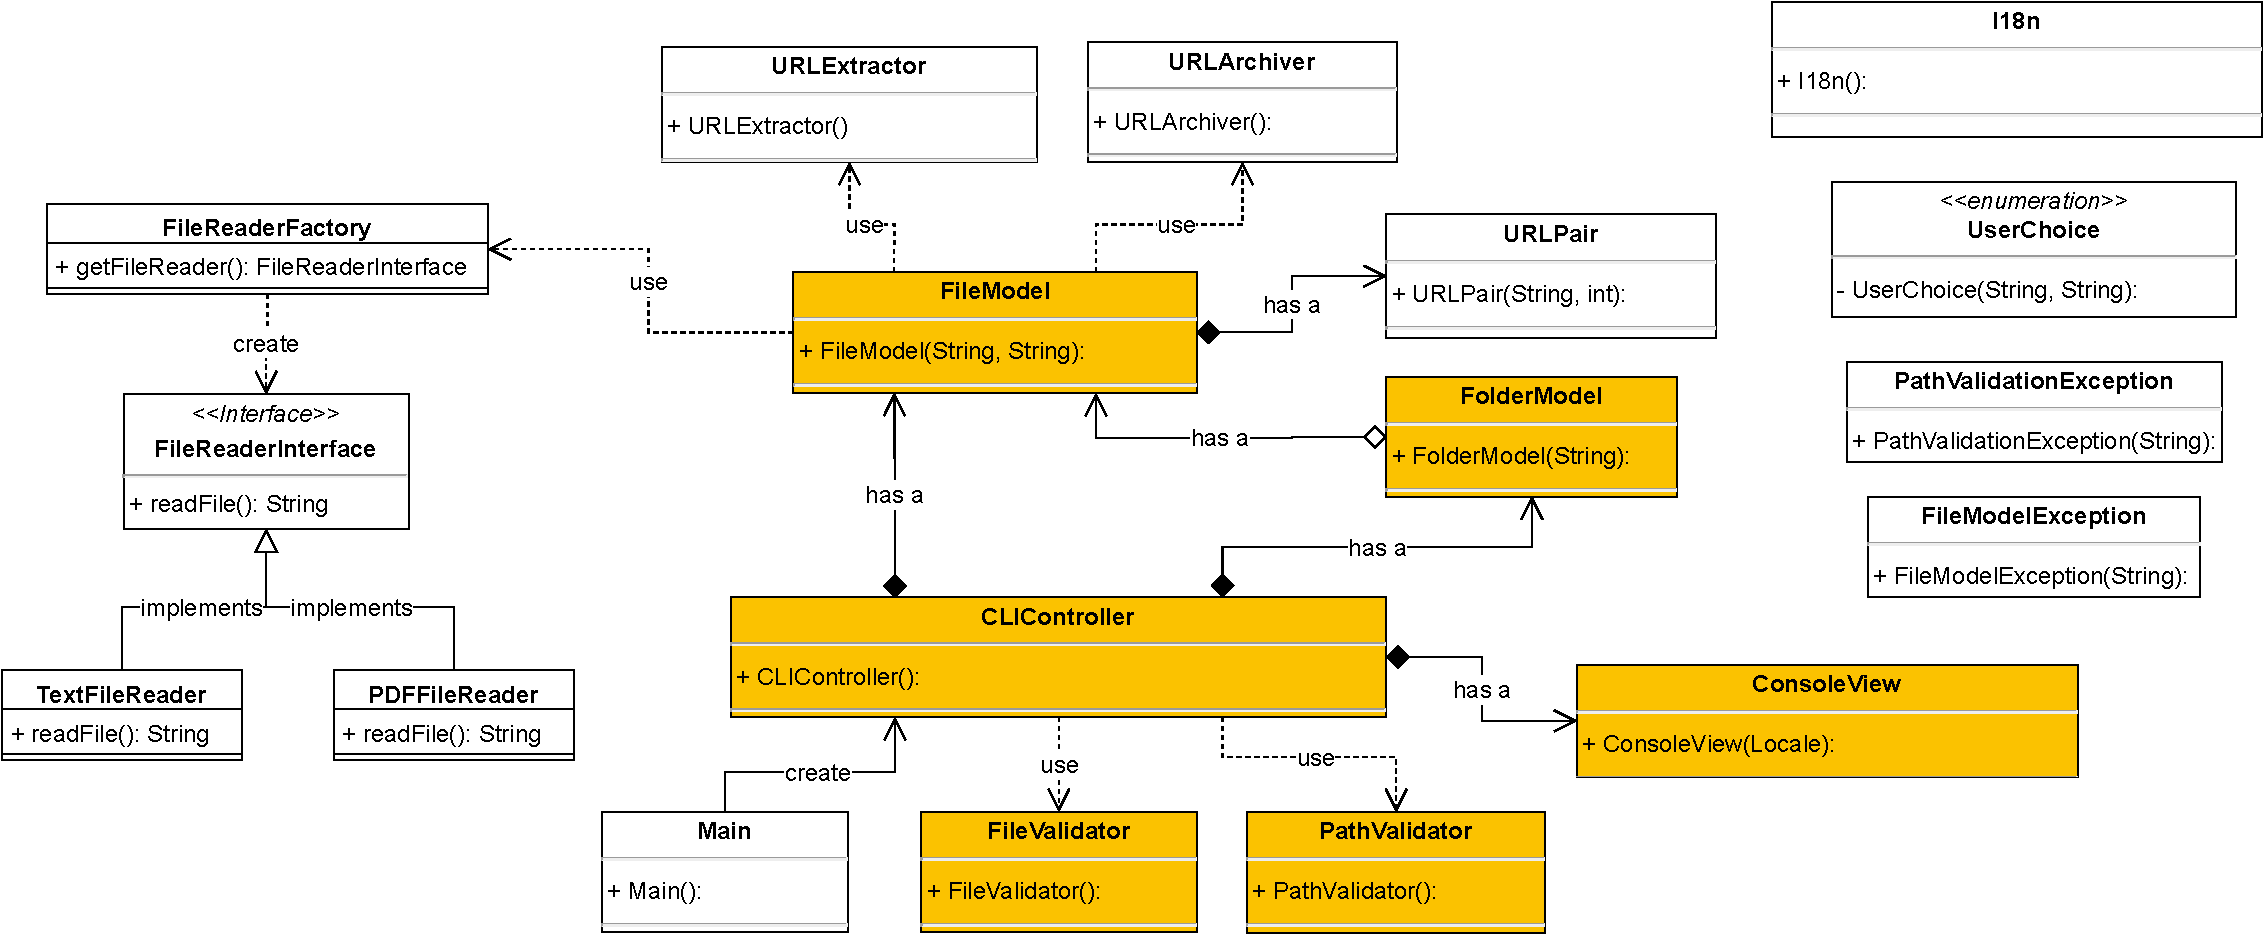
\includegraphics[width=1\textwidth]{pictures/URL_Archiver_Class_Diagram-Presentation_2}
%    \note{Now the controller...}
%    \note[item]{... checks the path and file type to avoid errors later.}
%    \note[item]{... decides whether to use a FolderModel or a FileModel based on what's given.}
%    \note[item]{... needs a ConsoleView to show the process on the screen for the user.}
%
%\end{frame}

% \begin{frame}{High Level Class Diagram}
%     \framesubtitle{FileModel}
%     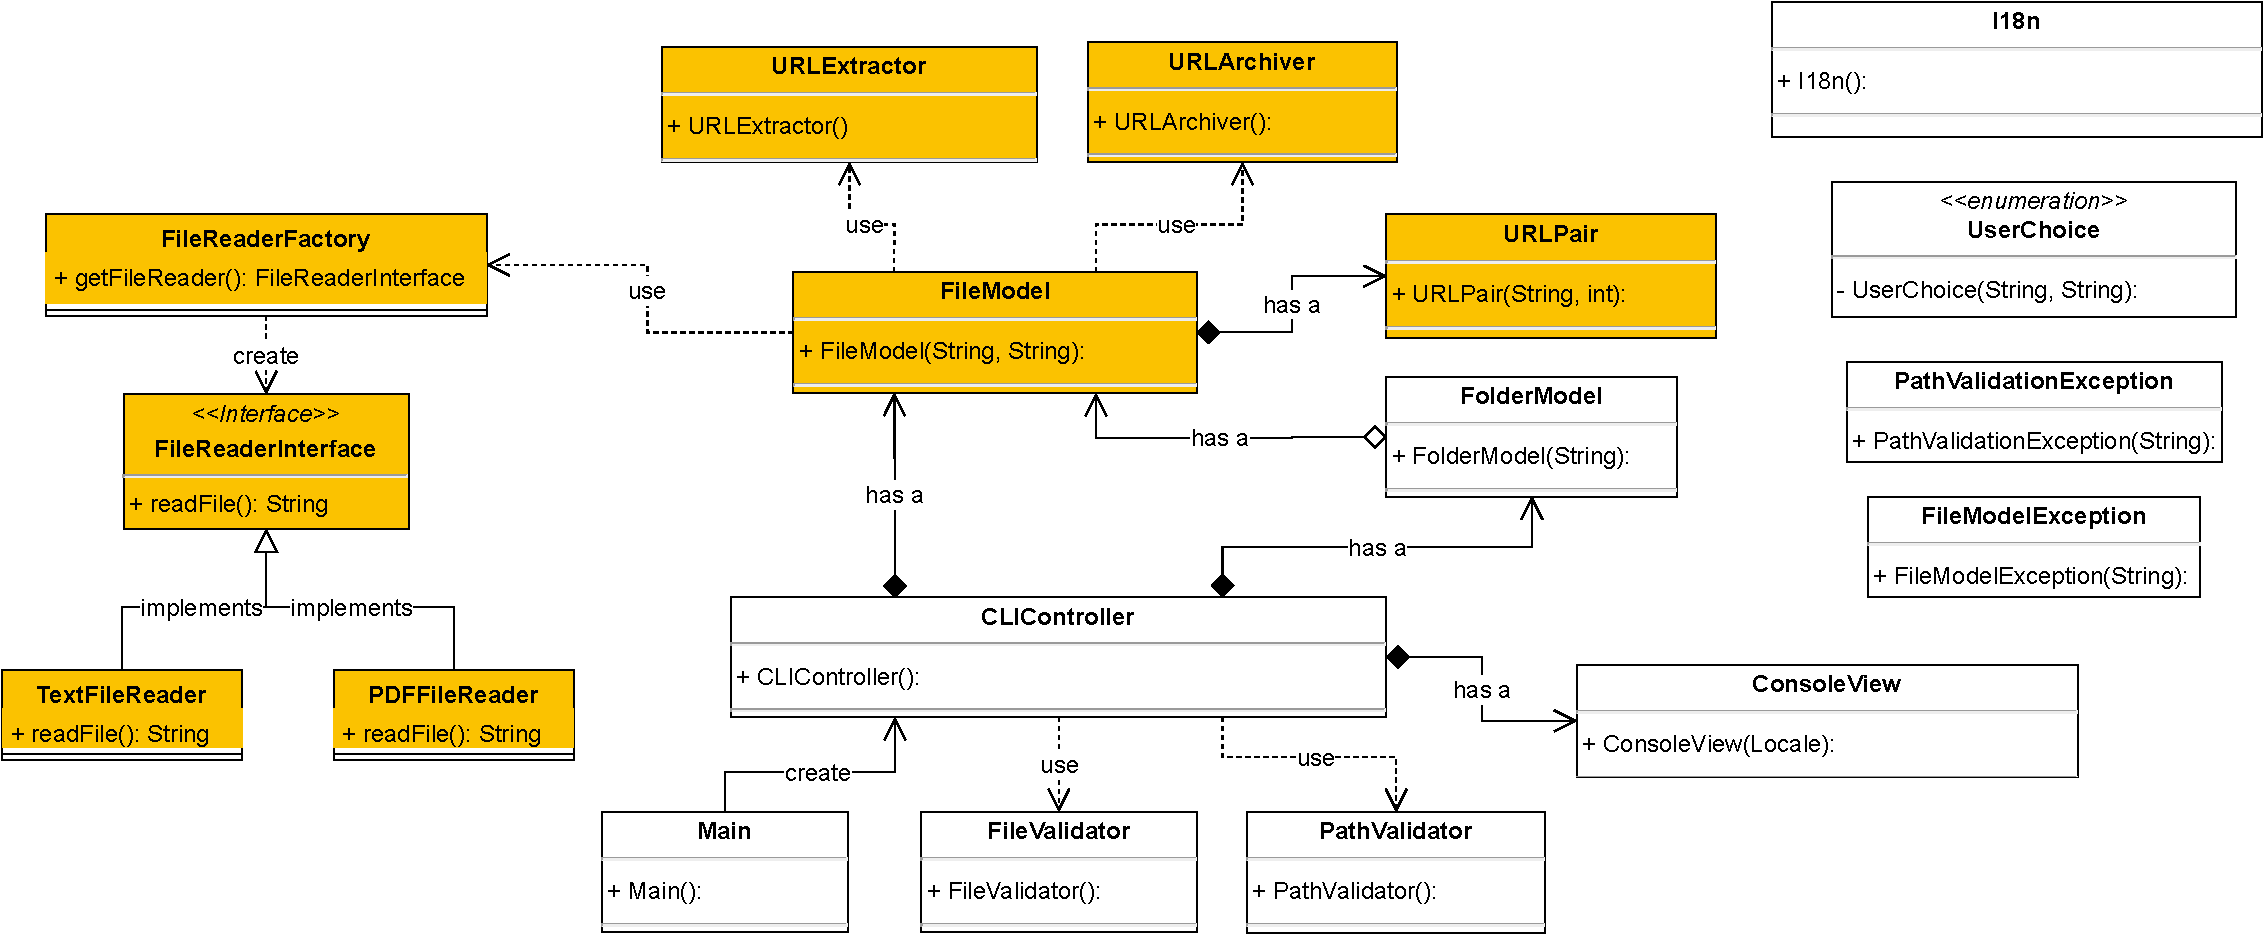
\includegraphics[width=1\textwidth]{pictures/URL_Archiver_Class_Diagram-Presentation_3}
%     \note[item]{Here you can see the data model where all the business logic takes place. However, I will be going into more detail about this later on, so I will refrain from going into any more detail at this point. }
% \end{frame}

%\begin{frame}{High Level Class Diagram}
%    \framesubtitle{I18n and UserChoice}
%    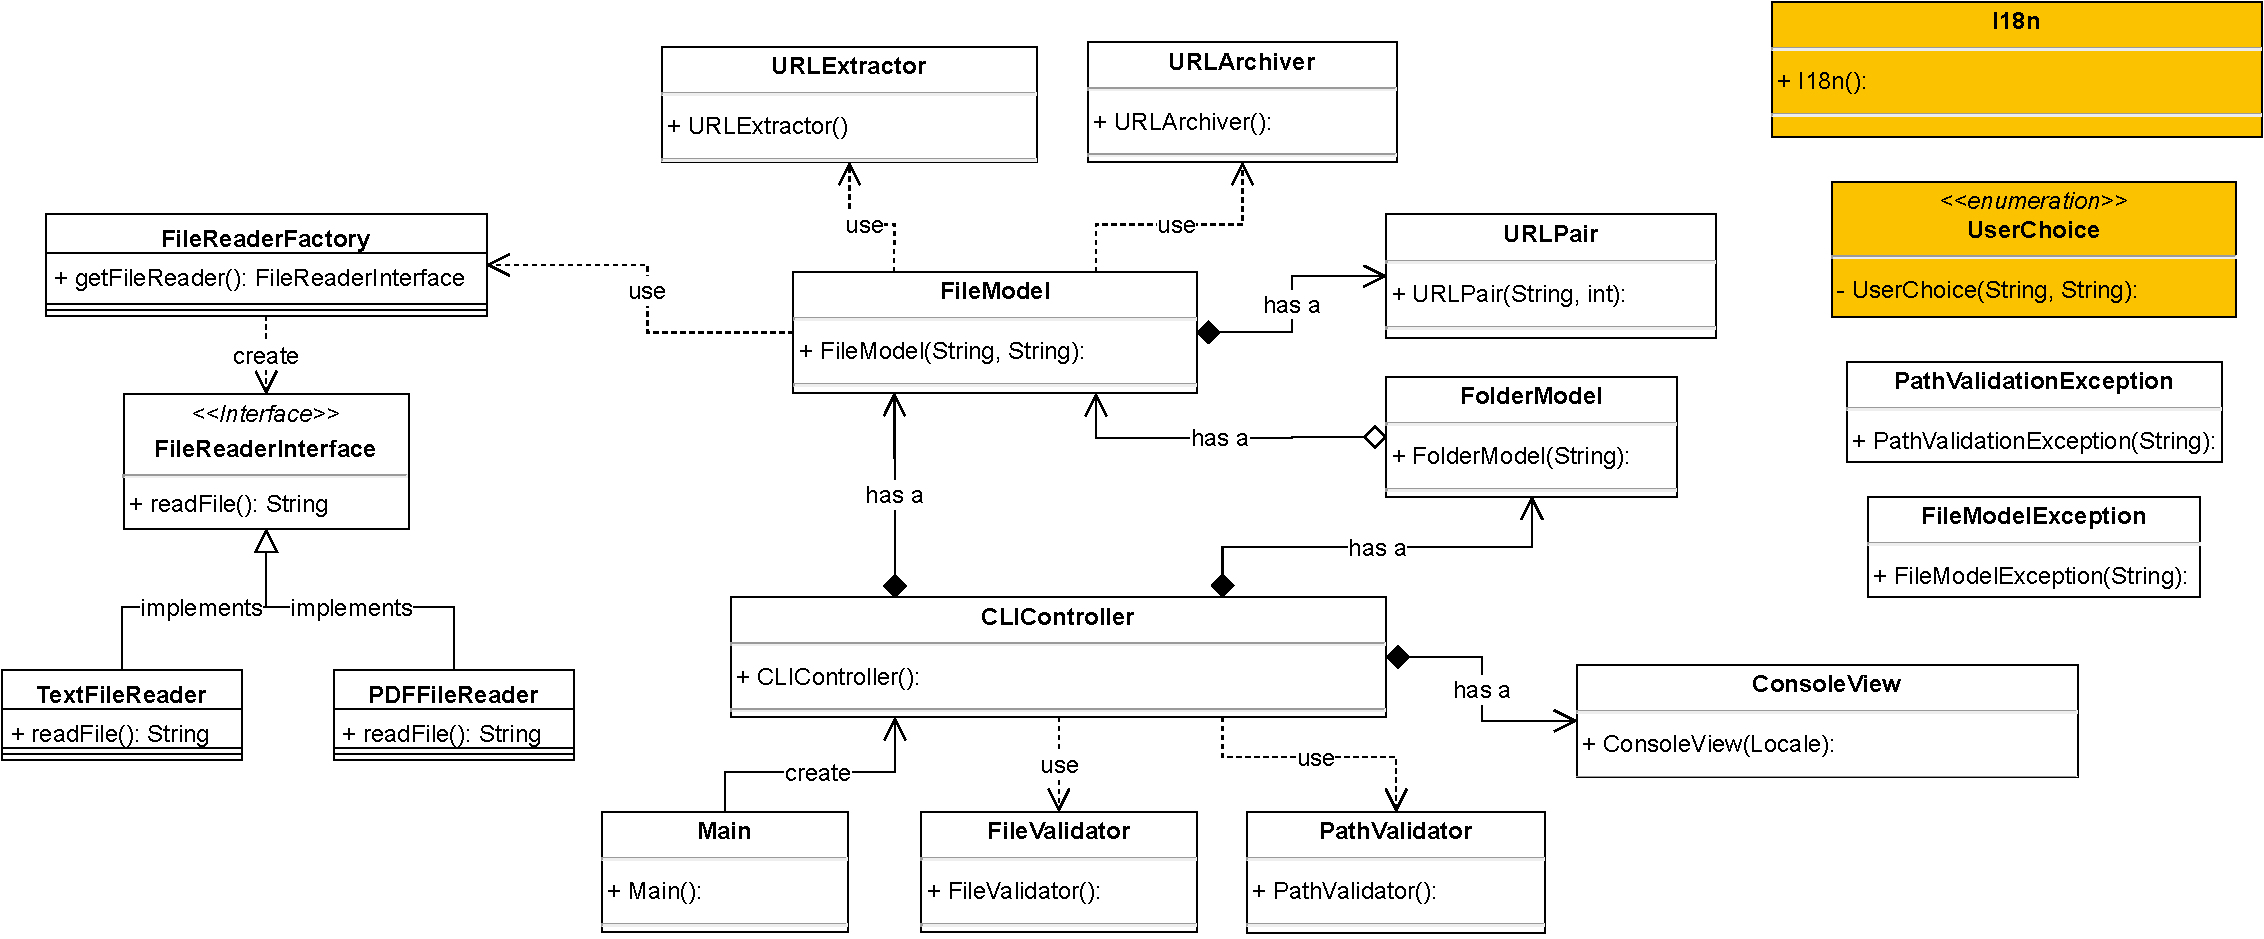
\includegraphics[width=1\textwidth]{pictures/URL_Archiver_Class_Diagram-Presentation_4}
%    \note[item]{Our application is ready for multiple languages, thanks to the I18n class. Right now, it's set up for English, but we can easily add more languages.}
%    \note[item]{We use the 'UserChoice' enum in conjunction with I18n to process user commands. While it's all in English at the moment, it's built to adapt to other languages without any hassle. }
%    \note[item]{By using I18n and UserChoice, we ensure a better experience for users and make our application flexible for international use in the future.}
%\end{frame}
%
%\begin{frame}{High Level Class Diagram}
%    \framesubtitle{Exceptions}
%    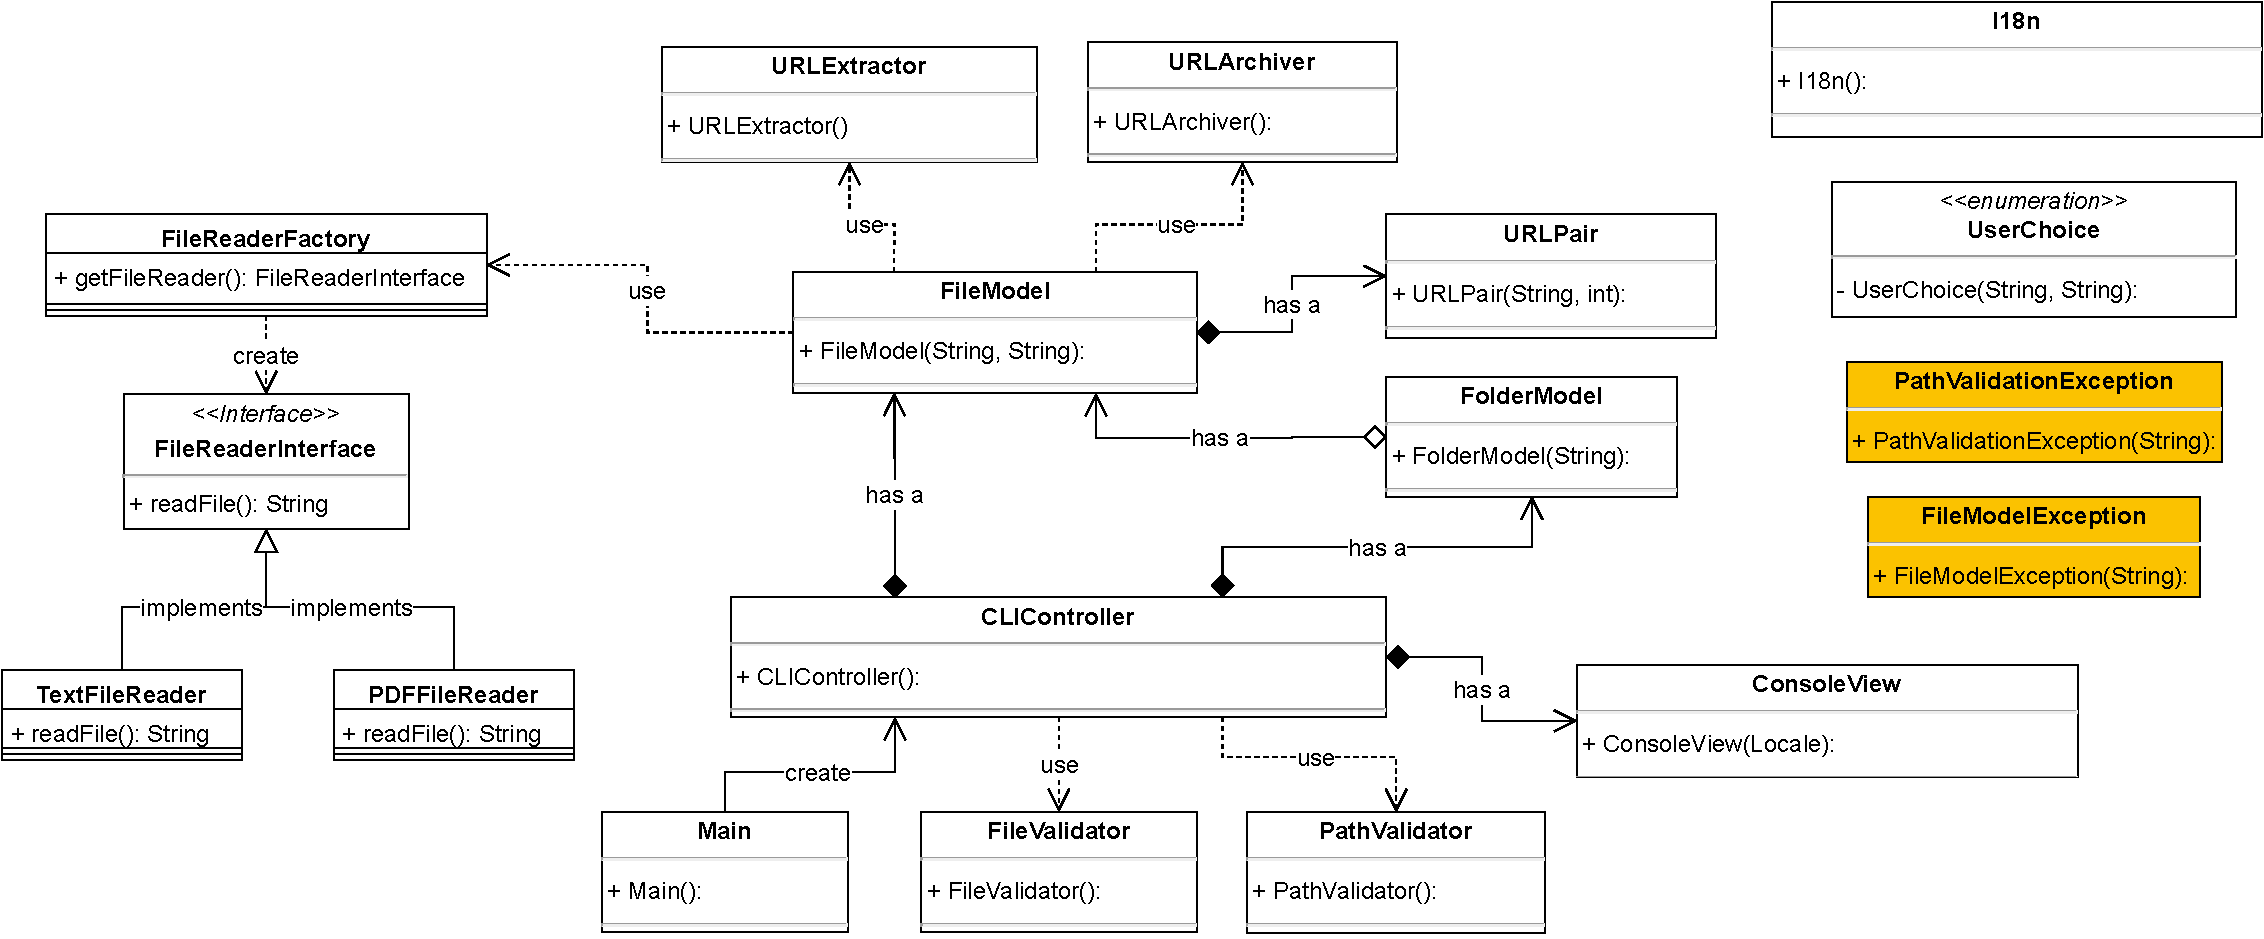
\includegraphics[width=1\textwidth]{pictures/URL_Archiver_Class_Diagram-Presentation_5}
%    \note[item]{Additionally, we have created our own exceptions for validating files and paths to enhance user experience.  }
%\end{frame}

    \begin{frame}{Architecture}
        \framesubtitle{Factory Pattern}
        \begin{columns} % Start the columns environment
            \begin{column}{0.6\textwidth} % Define the width of the left column
                \begin{itemize}
                    \item \textbf{Scalable} and \textbf{robust} design
                    \item Ensures \textbf{maintainability} and clear code structure
                    \item Commitment to \textbf{best programming practices}
                \end{itemize}
            \end{column}
            \begin{column}{0.4\textwidth} % Define the width of the right column
                \begin{center}
                    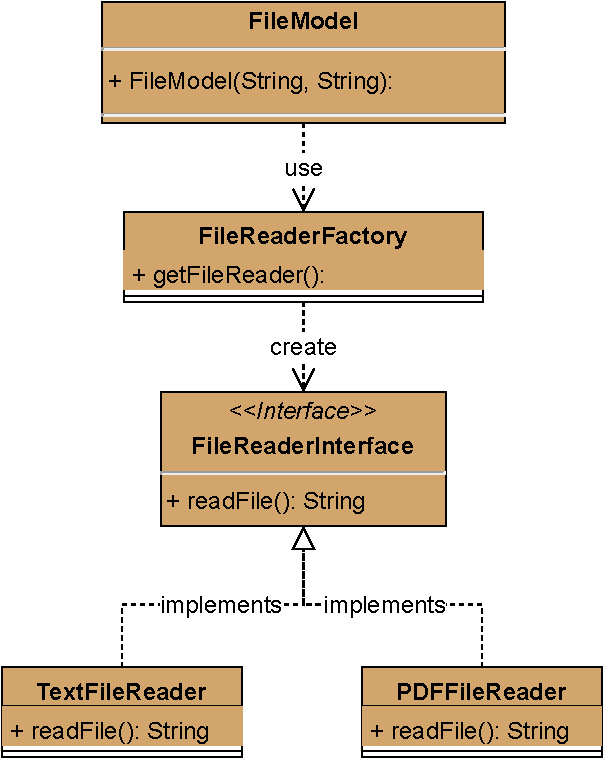
\includegraphics[width=0.7\textwidth]{figures/URL_Archiver_Class_Diagram-FileReaderFactory}
                \end{center}
            \end{column}
        \end{columns} % End the columns environment
        \note[item]{To enhance our application's flexibility further, we've implemented a factory class that reads and processes different file formats. }
        \note[item]{With a single call to the getFileReader() method from the FileReaderFactory, specifying the file type, we retrieve an appropriate FileReader. }
        \note[item]{Currently, our application can handle all UNICODE text files and PDFs.}
    \end{frame}

%  \begin{frame}{Architecture}
%      \framesubtitle{Multilanguage Support with ResourceBundle}
%      \begin{columns} % Start the columns environment
%          \begin{column}{0.6\textwidth} % Define the width of the left column
%              \begin{itemize}
%                  \item Ready for global adaptability.
%                  \item Future-proofing architectural choice.
%                  \item Potential to accommodate multiple languages.
%              \end{itemize}
%          \end{column}
%          \begin{column}{0.4\textwidth} % Define the width of the right column
%              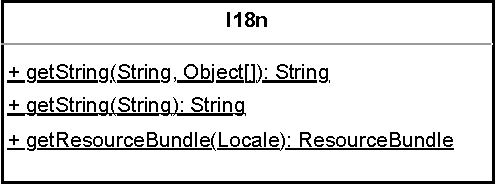
\includegraphics[width=0.7\textwidth]{pictures/URL_Archiver_Class_Diagram-I18n}
%          \end{column}
%      \end{columns} % End the columns environment
%  \end{frame}


% Slide for Key Components

    \subsection{Data Model}
    \begin{frame}{Key Components of the Data Model}
        \framesubtitle{Overview}
        \begin{columns} % Start the columns environment
            \begin{column}{0.5\textwidth} % Define the width of the left column
                \begin{itemize}
                    \item \textbf{FileModel}: Represents and handles individual files
                    \item \textbf{FolderModel}: Manages a collection of FileModel instances
                    \item \textbf{URLPair}: Links extracted URLs with their archived counterparts
                    \item \textbf{FileReaderFactory}: Organizes and maintains URLPairs
                    \item \textbf{URLExtractor}: Used for URL extraction
                    \item \textbf{URLArchiver}: Used for URL archiving
                \end{itemize}
            \end{column}
            \begin{column}{0.5\textwidth} % Define the width of the right column
                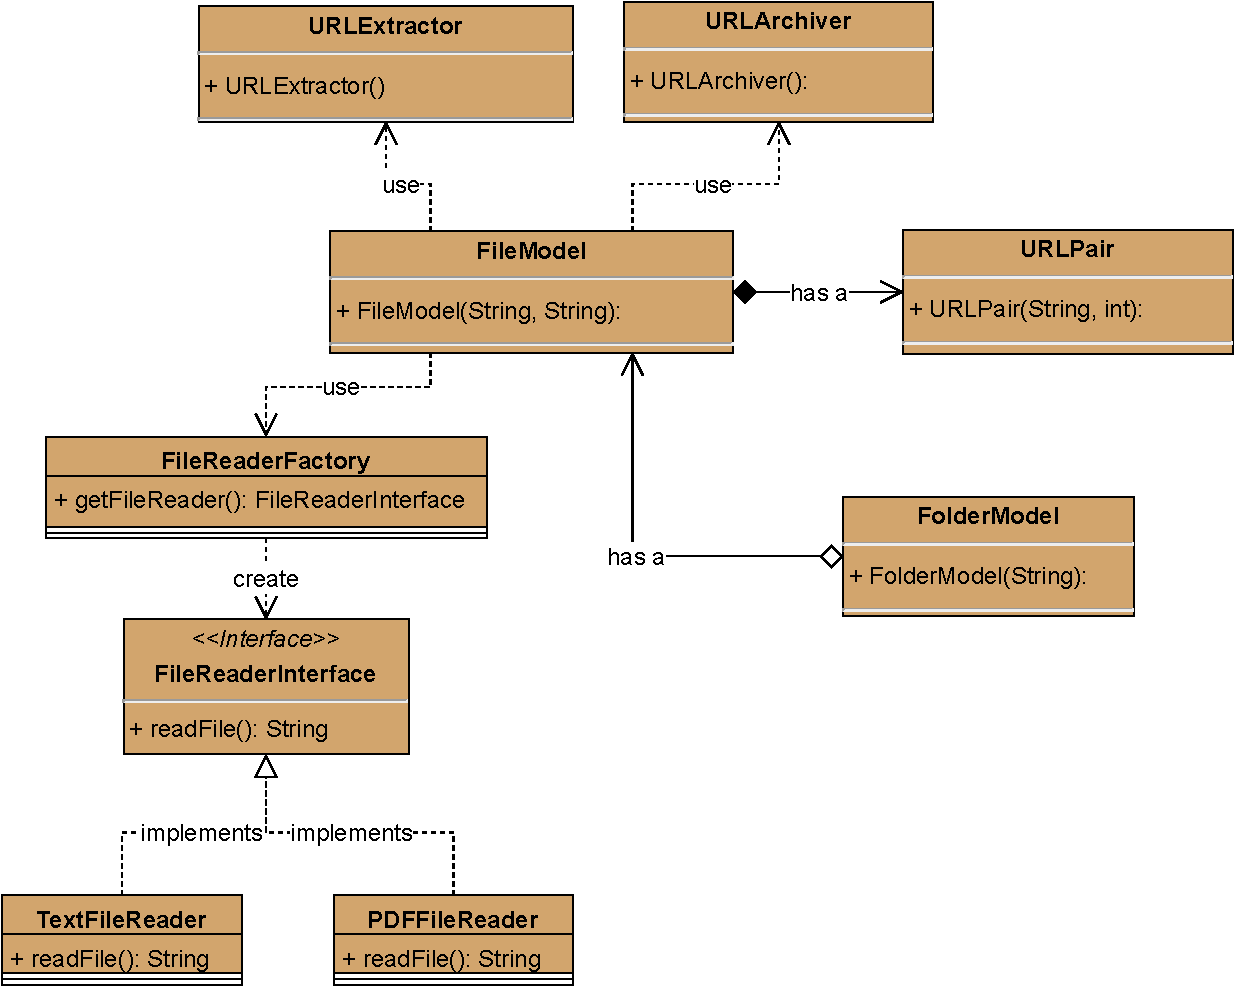
\includegraphics[width=1\textwidth]{figures/URL_Archiver_Class_Diagram-DataModel}
            \end{column}
        \end{columns} % End the columns environment
        \note{Now, let us discuss our data model. It is consists of the following classes:}
        \note[item]{The FileModel class manages the details of individual files. Each FileModel potentially containing multiple URLPair objects.}
        \note[item]{The FolderModel is applied when a user provides a folder path, storing the folder's structure and containing a list of FileModel objects.}
        \note[item]{The FileReaderFactory is our system for providing the right reader for a file, based on its type. This ensures that each file is read correctly and efficiently.}
        \note[item]{With the URLExtractor, our model extracts URLs from text, and the URLArchiver takes care of the URL archiving process.}
        \note[item]{This setup not only facilitates a clear division of tasks among the different components but also streamlines the process of archiving and retrieving URLs.}
        \note[item]{And now to the technologies we use for development.}
    \end{frame}

%\begin{frame}{Data Model}
%    \framesubtitle{FolderModel Class}
%    \begin{columns} % Start the columns environment
%        \begin{column}{0.5\textwidth} % Define the width of the left column
%            \begin{itemize}
%                \item Utilized upon user-defined folder path.
%                \item Stores folder structure within FolderModel.
%                \item Contains list of FileModel objects.
%                \item Essential for archiving URLs into .BIB files.
%                \item Facilitates clear division of responsibilities.
%            \end{itemize}
%        \end{column}
%        \begin{column}{0.5\textwidth} % Define the width of the right column
%            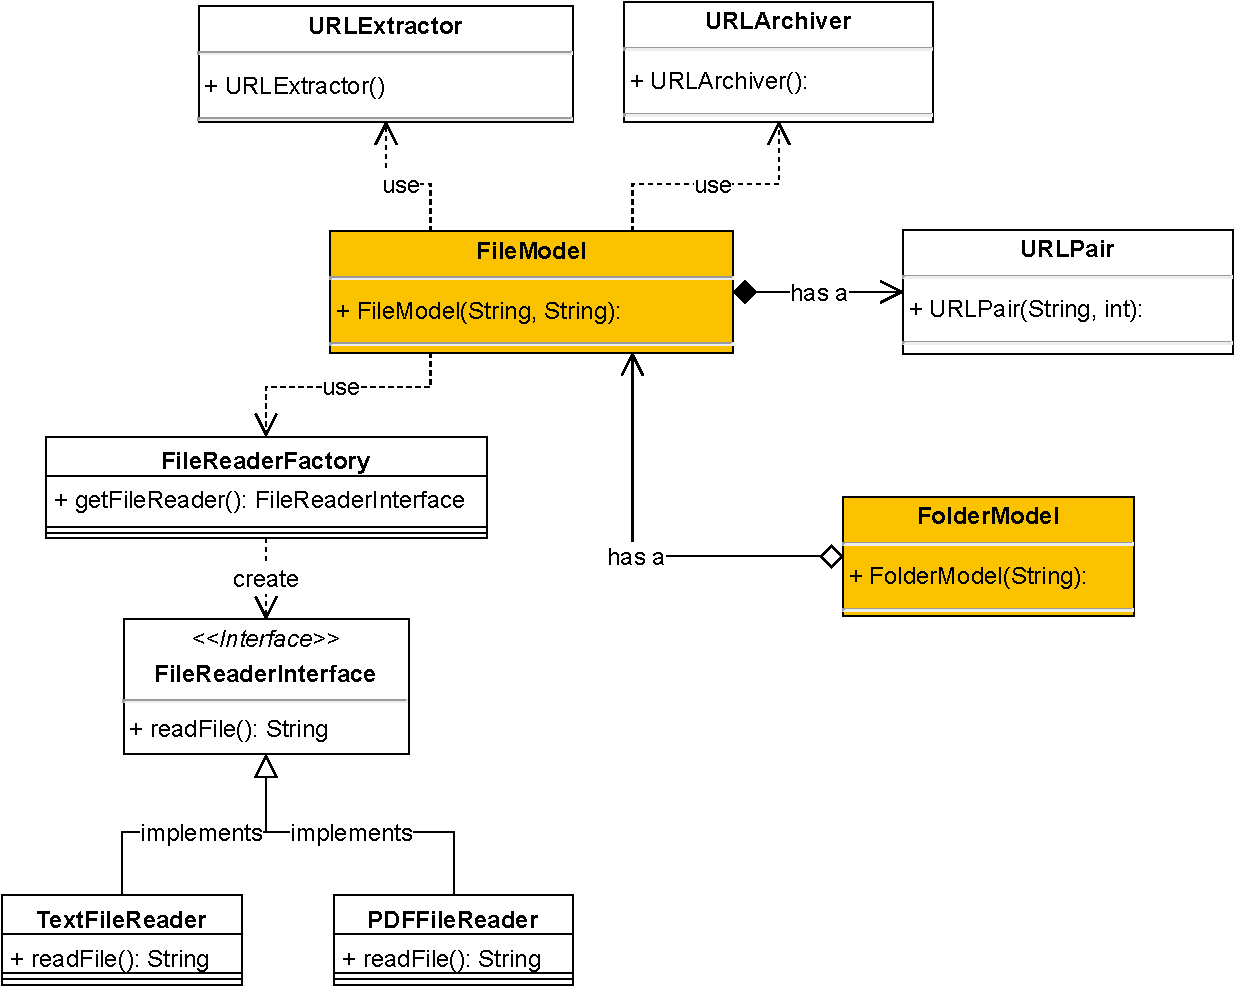
\includegraphics[width=1\textwidth]{pictures/URL_Archiver_Class_Diagram-DataModel_1}
%        \end{column}
%    \end{columns} % End the columns environment
%    \note{The FolderModel class is only used when the user specifies a path to a folder. In such a case, the structure of the folder is stored in the FolderModel, i.e. there is a list of FileModel objects. }
%    \note[item]{This will be important later when the archive URLs are written back to a file (.BIB).}
%    \note[item]{It also allows us to separate the responsibilities nicely.  }
%\end{frame}
%
%\begin{frame}{Data Model}
%    \framesubtitle{FileModel Class}
%    \begin{columns} % Start the columns environment
%        \begin{column}{0.5\textwidth} % Define the width of the left column
%            \begin{itemize}
%                \item FileModel operates independently or within FolderModel.
%                \item Stores list of URLPair objects.
%                \item Utilizes FileReaderFactory to select appropriate reader.
%                \item Extracts and saves URLs using URLExtractor.
%                \item Archives URLs upon user's command with URLArchiver.
%            \end{itemize}
%        \end{column}
%        \begin{column}{0.5\textwidth} % Define the width of the right column
%            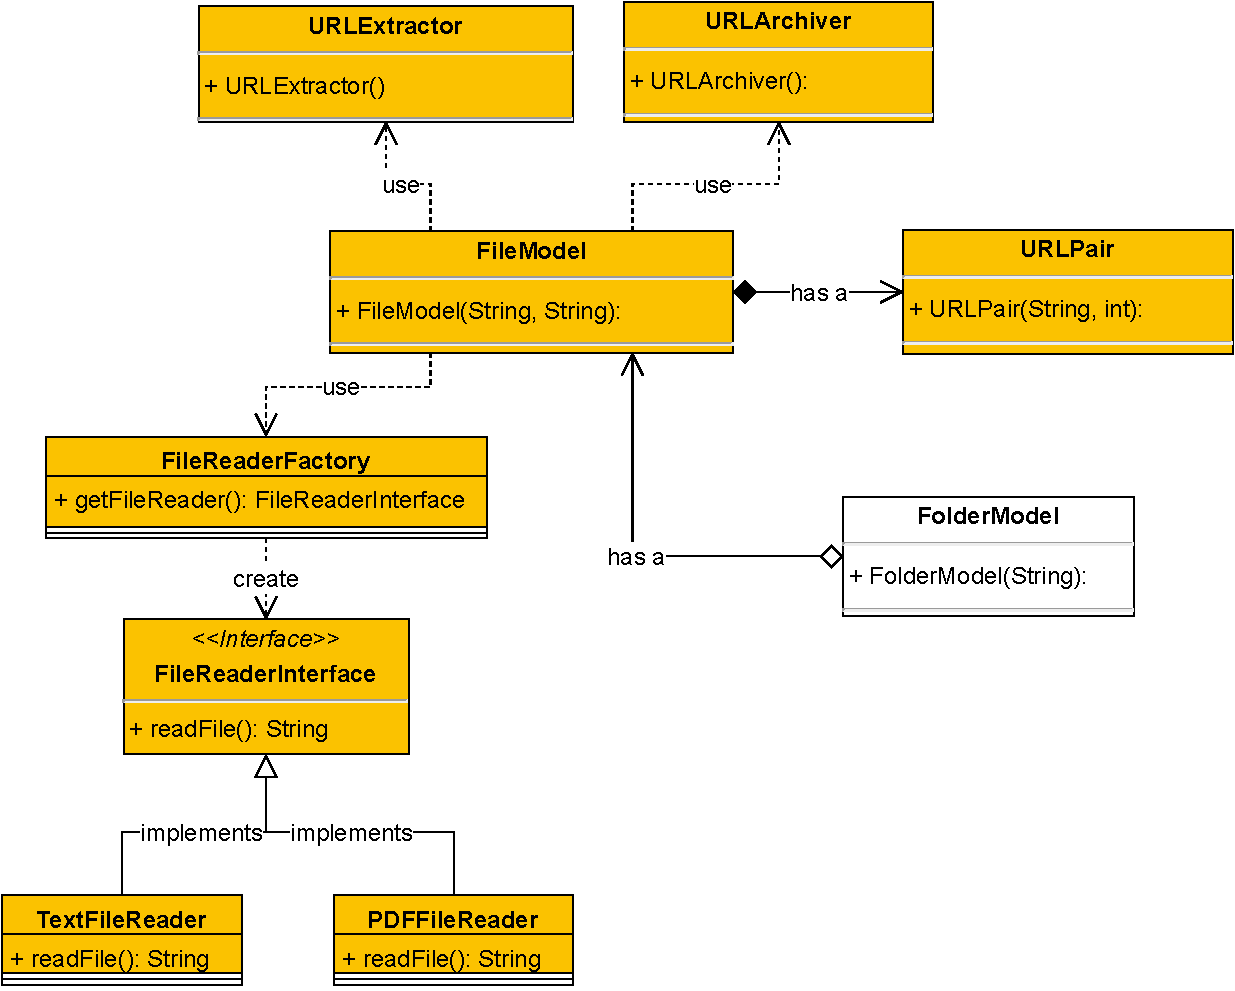
\includegraphics[width=1\textwidth]{pictures/URL_Archiver_Class_Diagram-DataModel_2}
%        \end{column}
%    \end{columns} % End the columns environment
%    \note[item]{The FileModel class can exist without a FolderModel class.}
%    \note[item]{This is the case when the user specifies only one file.}
%    \note[item]{In any case, the FileModel class is currently responsible for storing a list of URLPairs objects. }
%    \note[item]{It also uses a reader to read the text from the file; the necessary reader is provided by the FileReaderFactory, depending on the file type.}
%    \note[item]{It then uses the URLExtractor to read the URLs from the text and store them in a URLPair. If the user wants to archive the URL, it uses the URLArchiver. }
%\end{frame}

    \subsection{Technologies}
    \begin{frame}{Technologies I/II}
        \begin{columns}
            \begin{column}{0.7\textwidth}
                \begin{itemize}
                    \item \textbf{Java}: The primary programming language for our application
                    \item \textbf{LaTeX}: Used for documentation and presentation
                    \item \textbf{JUnit 5}: Utilized for unit testing
                    \item \textbf{PDFTextStripper (PDFBox library)}: Used for extracting text from PDF documents
                    \item \textbf{Selenium}: Web automation tool used for tasks like inputting URLs, handling \textbf{captchas}, and retrieving archived URLs due to the absence of an official API from archive.today
                    \item \textbf{Maven}: Essential for compilation, dependency management, and building the project
                \end{itemize}

                \note[item]{The application is developed in Java, while the report, presentations, and user manual are authored in LaTeX.}
                \note[item]{For testing, we utilize JUnit 5, and for text extraction from PDFs, we rely on PDFTextStripper. }
                \note[item]{The archiving process on Archive.today is executed using Selenium to navigate the lack of an API and to address captcha challenges.}
                \note[item]{Additionally, we use Maven for building the application and managing dependencies.}
            \end{column}

            \begin{column}{0.3\textwidth}
                
\includegraphics[height=0.5cm]{pictures/Java-Logo}
                \vspace{1em}
                
\includegraphics[height=0.5cm]{pictures/LaTeX_logo}
                \vspace{1em}
                
\includegraphics[height=0.5cm]{pictures/JUnit_5_Logo}
                \vspace{1em}
                
\includegraphics[height=0.5cm]{pictures/Apache_PDFBox_logo}
                \vspace{1em}
                
\includegraphics[height=0.5cm]{pictures/Selenium_logo}
                \vspace{1em}
                
\includegraphics[height=0.5cm]{pictures/Apache_Maven_logo}
            \end{column}
        \end{columns}
    \end{frame}

    \begin{frame}{Technologies II/II}
        \begin{columns}
            \begin{column}{0.7\textwidth}
                \begin{itemize}
                    \item \textbf{Archive.today}: One of the services used by the URL-Archiver to archive URLs
                    \item \textbf{Wayback Machine}: One of the services used by the URL-Archiver to archive URLs
                    \item \textbf{JetBrains IntelliJ IDEA}: Used to develop the program and create the report and presentation in Latex
                    \item \textbf{GitHub}: A platform for code hosting and collaboration, allowing us to manage our program's development and version control
                    \item \textbf{Atlassian Jira}: A tool for tracking progress and managing our project goals and tasks
                \end{itemize}
            \end{column}
            \begin{column}{0.3\textwidth}
                
\includegraphics[height=1cm]{pictures/Wayback_Machine_logo}
                \vspace{1em}
                \includegraphics[height=1cm]{pictures/archive_today_logo}
                \vspace{1em}
                \includegraphics[height=1cm]{pictures/IntelliJ_IDEA_Icon}
                \vspace{1em}
                \includegraphics[height=1cm]{pictures/github-mark}
                \vspace{1em}
                \includegraphics[height=1cm]{pictures/jira_logo}
            \end{column}
        \end{columns}
        \note[item]{Furthermore, we rely on Archive.today and additionally on the Wayback Machine to archive URLs.}
        \note[item]{As our development environment, we use JetBrains' IntelliJ IDEA.}
        \note[item]{We use Github to store our code and for version control. }
        \note[item]{To manage and plan our project, we use Jira.}
    \end{frame}

%-------------------------------%

% Chapter two "Project Management with SCRUM"


    \section{Project Management with SCRUM}
    \setbeamertemplate{section page}[BFH-ruled]
    \frame{\sectionpage}

    \subsection{Scrum Team}
% Experiment Slide
    \begin{frame}{Our Scrum Team}
        \begin{center}
% First member
            \begin{minipage}{.3\textwidth}
                \centering
                \hexagonimage{pictures/dora_2} \\ % Replace with the correct file name
                \textbf{Nicolin Dora}\\
                Product Owner \& Developer
            \end{minipage}
% Second member
            \begin{minipage}{.3\textwidth}
                \centering
                \hexagonimage{pictures/vejseli_2}\\ % Replace with the correct file name
                \textbf{Abidin Vejseli}\\
                Scrummaster \& Developer
            \end{minipage}
% Third member
            \begin{minipage}{.3\textwidth}
                \centering
                \hexagonimage{pictures/wampfler_2}\\ % Replace with the correct file name
                \textbf{Kilian Wampfler}\\
                Developer
            \end{minipage}
        \end{center}
    \end{frame}

% Experiment Slide
    \begin{frame}{Other Roles}
        \begin{center}
% First member
            \begin{minipage}{.3\textwidth}
                \centering
                \hexagonimage{pictures/kramer_2} \\ % Replace with the correct file name
                \textbf{Dr. Simon Kramer}\\
                Stakeholder \& Customer
            \end{minipage}
% Second member
            \begin{minipage}{.3\textwidth}
                \centering
                \hexagonimage{pictures/helbling_2}\\ % Replace with the correct file name
                \textbf{Frank Helbling}\\
                PM-Advisor
            \end{minipage}
        \end{center}
    \end{frame}

    \subsection{Our Scrum Adaptions}
    \begin{frame}{Our Scrum Adaptions}
        \framesubtitle{Sprint}
        \includegraphics[width=1\textwidth]{figures/scrum_adaptions-Sprint}
    \end{frame}

    \begin{frame}{Our Scrum Adaptions}
        \framesubtitle{Sprint Planning}
        \includegraphics[width=1\textwidth]{figures/scrum_adaptions-Sprint_Planning}
    \end{frame}

    \begin{frame}{Our Scrum Adaptions}
        \framesubtitle{Daily Scrum}
        \includegraphics[width=1\textwidth]{figures/scrum_adaptions-Daily_Scrum}
    \end{frame}

    \begin{frame}{Our Scrum Adaptions}
        \framesubtitle{Sprint Review}
        \includegraphics[width=1\textwidth]{figures/scrum_adaptions-Sprint_Review}
    \end{frame}

    \begin{frame}{Our Scrum Adaptions}
        \framesubtitle{Sprint Retro}
        \includegraphics[width=1\textwidth]{figures/scrum_adaptions-Sprint_Retro}
    \end{frame}

    \subsection{Scrum implementation}
    \begin{frame}{Estimation Method}
        \framesubtitle{T-Shirt Sizes}
        \begin{center}
            \includegraphics[width=0.6\textwidth]{pictures/tshirt_sizes}
        \end{center}
    \end{frame}

    \begin{frame}{Velocity}
        \begin{center}
            \includegraphics[width=1\textwidth]{pictures/GANT-Diagramm}
        \end{center}
    \end{frame}

    \begin{frame}{Backlog}
        \begin{center}
            \includegraphics[width=1\textwidth]{pictures/Backlog 1}
        \end{center}
    \end{frame}

    \begin{frame}{Epics}
        \begin{center}
            \includegraphics[width=0.8\textwidth]{pictures/Epic}
        \end{center}
    \end{frame}

    \begin{frame}{Spint 2}
        \framesubtitle{Sprint Goal}
        \includegraphics[width=1\textwidth]{pictures/SprintBacklog 1}
    \end{frame}

    \begin{frame}{Spint 2}
        \framesubtitle{Categories}
        \includegraphics[width=1\textwidth]{pictures/Sprint Backlog 2}
    \end{frame}

    \begin{frame}{User Story}
        \framesubtitle{Description, Acceptance Criteria, DOR and DOD}
        \begin{center}
            \includegraphics[width=1\textwidth]{pictures/User Story 1}
        \end{center}
    \end{frame}

    \begin{frame}{Our learnings}
        \begin{columns}
            \begin{column}{0.5\textwidth}
                \begin{center}
                    \includegraphics[width=0.8\textwidth]{pictures/scrum_adaptions-learnings}
                \end{center}
            \end{column}
            \begin{column}{0.5\textwidth}
                \begin{center}
                    \includegraphics[width=0.8\textwidth]{pictures/Learnings}
                \end{center}
            \end{column}
        \end{columns}
    \end{frame}


%----------------------------------------%


    \section{Questions?}
    \setbeamertemplate{section page}[BFH-ruled]
    \frame{\sectionpage}

%-------------------------------%


%These can be automaticlly called by using \AtBeginSection{\sectionpage}

%Change base color scheme (option can be added)

%\setbeamercolor{BFH}{parent=BFH-Orange}

%\frame{\sectionpage}

%\setbeamertemplate{section page}[BFH]

%\frame{\sectionpage}

\end{document}

